\chapter{PHÂN TÍCH HỆ THỐNG}
\label{ch:system-analysis}

\section{Tổng quan Phân tích Hệ thống}
\label{sec:system-analysis-overview}

Chương này trình bày phân tích chi tiết hệ thống DSA Visualizer Platform từ góc độ kiến trúc phần mềm và thiết kế hệ thống. Phân tích được thực hiện thông qua các mô hình UML chuẩn bao gồm Use Case Diagram, Class Diagram, Activity Diagram, và Sequence Diagram, nhằm mô tả đầy đủ các yêu cầu chức năng, tương tác người dùng, và kiến trúc hệ thống.

\section{Use Case Diagram và Phân tích}
\label{sec:use-case-diagram}

\subsection{Tổng quan Use Case System}
\label{subsec:use-case-system-overview}

Hệ thống DSA Visualizer Platform được thiết kế để phục vụ ba nhóm actor chính với các vai trò và quyền hạn khác nhau:

\begin{itemize}
    \item \textbf{Sinh viên (Học viên)}: Nhóm người dùng chính, sử dụng nền tảng để học tập thuật toán
    \item \textbf{Giảng viên (Người hướng dẫn)}: Quản lý nội dung học tập, tạo bài tập và theo dõi tiến độ học viên
    \item \textbf{Quản trị viên (Người quản lý)}: Quản lý hệ thống, người dùng và duy trì hoạt động nền tảng
\end{itemize}

Ngoài ra, hệ thống tương tác với các hệ thống bên ngoài để cung cấp các dịch vụ hỗ trợ:

\begin{itemize}
    \item \textbf{Hệ thống AI}: Cung cấp hỗ trợ học tập thông minh
    \item \textbf{Hệ thống Cơ sở dữ liệu}: Lưu trữ và quản lý dữ liệu
    \item \textbf{Dịch vụ Thông báo}: Gửi thông báo và cảnh báo
    \item \textbf{Dịch vụ Phân tích}: Thu thập và phân tích dữ liệu học tập
\end{itemize}

\begin{figure}[H]
\centering
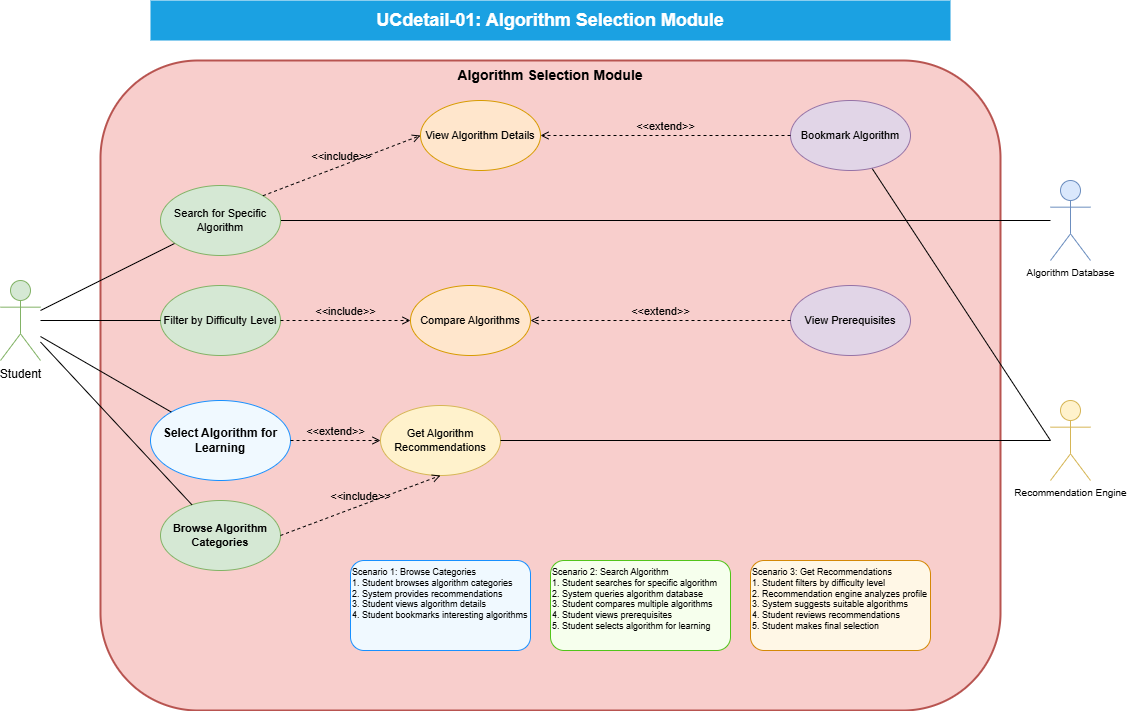
\includegraphics[width=1.0\textwidth]{enhanced-diagrams/UCdetail-01-algorithm-selection.png}
\caption{Sơ đồ Use Case - Tổng quan Hệ thống}
\label{fig:usecase-system-overview}
\end{figure}

\subsection{Phân nhóm Use Case theo Chức năng}
\label{subsec:use-case-functional-groups}

Các use case được tổ chức thành 4 nhóm chức năng chính:

\subsubsection{Nhóm Học Tập Sinh Viên (5 ca sử dụng)}
\begin{enumerate}
    \item \textbf{Học Khái Niệm Thuật Toán}: Học các khái niệm thuật toán cơ bản
    \item \textbf{Thực Hành Với Hình Ảnh Hóa}: Thực hành với animation tương tác
    \item \textbf{Thực Hiện Đánh Giá}: Thực hiện các bài kiểm tra đánh giá
    \item \textbf{Theo Dõi Tiến Độ Học Tập}: Theo dõi tiến độ học tập cá nhân
    \item \textbf{Hợp Tác Với Đồng Học}: Tương tác và học tập cùng đồng học
\end{enumerate}

\subsubsection{Nhóm Quản Lý Giảng Viên (4 ca sử dụng)}
\begin{enumerate}
    \item \textbf{Quản Lý Nội Dung Học Tập}: Quản lý nội dung học tập và tài liệu
    \item \textbf{Tạo Bài Đánh Giá}: Tạo các bài kiểm tra và quiz
    \item \textbf{Theo Dõi Tiến Độ Sinh Viên}: Theo dõi tiến độ học tập của học viên
    \item \textbf{Quản Lý Lớp Học}: Quản lý lớp học và nhóm học viên
\end{enumerate}

\subsubsection{Nhóm Quản Trị Hệ Thống (4 use cases)}
\begin{enumerate}
    \item \textbf{Quản lý Người dùng Hệ thống}: Quản lý tài khoản và quyền người dùng
    \item \textbf{Bảo trì Hệ thống}: Bảo trì và cập nhật hệ thống
    \item \textbf{Giám sát Hiệu suất Hệ thống}: Giám sát hiệu suất hệ thống
    \item \textbf{Quản lý Bảo mật}: Quản lý bảo mật và quyền truy cập
\end{enumerate}
\end{enumerate>

\subsubsection{Nhóm Hỗ trợ Hệ thống Cốt lõi (5 use cases)}
\begin{enumerate}
    \item \textbf{Xác thực Người dùng}: Xác thực và quản lý phiên đăng nhập
    \item \textbf{Quản lý Dữ liệu}: Quản lý dữ liệu và lưu trữ
    \item \textbf{Hỗ trợ AI Thông minh}: Cung cấp hỗ trợ AI thông minh
    \item \textbf{Gửi Thông báo}: Gửi thông báo và cảnh báo
    \item \textbf{Tạo Báo cáo Phân tích}: Tạo báo cáo và phân tích dữ liệu
\end{enumerate}

\subsection{Đặc tả Chi tiết Use Case}
\label{subsec:detailed-usecase-specs}

Phần này trình bày chi tiết các use case chính của hệ thống theo format chuẩn academic, mô tả đầy đủ các luồng sự kiện, điều kiện tiên quyết, và kết quả mong đợi.

\subsubsection{UC001: Học tập Trực quan hóa Thuật toán}

\begin{usecase}
\addheading{Use Case ID}{UC001}
\addrow{Tên Use Case}{Học tập Trực quan hóa Thuật toán}
\addrow{Actor}{Sinh viên}
\addrow{Mô tả ngắn gọn}{Học viên học thuật toán thông qua trực quan hóa tương tác.}
\addrow{Trigger}{Học viên muốn học và hiểu thuật toán thông qua trực quan hóa.}
\addmulrow{Precondition}{\begin{itemize}
    \item Học viên đã đăng nhập vào hệ thống.
    \item Hệ thống có sẵn nội dung thuật toán.
    \item Trình duyệt hỗ trợ HTML5 Canvas/WebGL.
\end{itemize}}
\addmulrow{Main Flow}{\begin{enumerate}
    \item Học viên chọn loại thuật toán muốn học.
    \item Hệ thống hiển thị danh sách thuật toán có sẵn.
    \item Học viên chọn thuật toán cụ thể (VD: Quick Sort).
    \item Hệ thống tải giao diện trực quan hóa thuật toán.
    \item Học viên nhập dữ liệu hoặc sử dụng dữ liệu mẫu.
    \item Học viên bắt đầu quá trình trực quan hóa.
    \item Hệ thống thực hiện hoạt hình từng bước.
    \item Học viên điều khiển tốc độ, tạm dừng, tiếp tục theo nhu cầu.
    \item Hệ thống hiển thị phân tích độ phức tạp và giải thích.
    \item Học viên hoàn thành phiên học tập.
\end{enumerate}}
\addmulrow{Alternative Flow}{\textbf{Alt 1: Học viên muốn so sánh thuật toán}
\begin{itemize}
    \item Từ bước 3, học viên chọn nhiều thuật toán.
    \item Hệ thống hiển thị giao diện so sánh.
    \item Học viên chạy cùng lúc để so sánh hiệu suất.
\end{itemize}}
\addmulrow{Exception Flow}{\textbf{Exc 1: Dữ liệu đầu vào không hợp lệ}
\begin{itemize}
    \item Hệ thống hiển thị thông báo lỗi.
    \item Yêu cầu học viên nhập lại dữ liệu.
\end{itemize}
\textbf{Exc 2: Lỗi thực thi thuật toán}
\begin{itemize}
    \item Hệ thống đặt lại trực quan hóa.
    \item Hiển thị dữ liệu mẫu mặc định.
\end{itemize}}
\addmulrow{Post Condition}{\begin{itemize}
    \item Tiến độ học tập được cập nhật.
    \item Dữ liệu phiên được lưu trong hồ sơ.
    \item Dữ liệu phân tích được ghi nhận.
\end{itemize}}
\end{usecase}

\subsubsection{UC002: Thực hành Thuật toán Tương tác}

\begin{usecase}
\addheading{Use Case ID}{UC002}
\addrow{Tên Use Case}{Thực hành Thuật toán Tương tác}
\addrow{Actor}{Sinh viên}
\addrow{Mô tả ngắn gọn}{Học viên thực hành thuật toán với điều khiển tương tác và đầu vào tùy chỉnh để củng cố kiến thức.}
\addrow{Trigger}{Học viên muốn thực hành và kiểm tra hiểu biết về thuật toán đã học.}
\addmulrow{Precondition}{\begin{itemize}
    \item Học viên đã hoàn thành học tập trực quan hóa cơ bản.
    \item Môi trường thực hành được kích hoạt.
    \item Mẫu thuật toán có sẵn trong hệ thống.
\end{itemize}}
\addmulrow{Main Flow}{\begin{enumerate}
    \item Học viên chọn "Chế độ Thực hành" từ giao diện thuật toán.
    \item Hệ thống hiển thị danh sách thuật toán thực hành có sẵn.
    \item Học viên chọn thuật toán cụ thể để thực hành.
    \item Hệ thống tải môi trường thực hành tương tác với các điều khiển.
    \item Học viên tạo dữ liệu đầu vào tùy chỉnh hoặc chọn từ ví dụ có sẵn.
    \item Học viên dự đoán hành vi thuật toán trước khi thực thi.
    \item Học viên thực thi thuật toán với điều khiển từng bước.
    \item Hệ thống cung cấp phản hồi thời gian thực và gợi ý hiệu suất.
    \item Học viên so sánh dự đoán với kết quả thực thi thực tế.
    \item Hệ thống tính điểm thực hành và cung cấp đề xuất cải thiện.
\end{enumerate}}
\addmulrow{Alternative Flow}{\textbf{Alt 1: Chế độ Thực hành Hướng dẫn}
\begin{itemize}
    \item Hệ thống cung cấp gợi ý và hướng dẫn từng bước.
    \item Học viên được hỗ trợ với giải thích chi tiết cho mỗi bước.
\end{itemize}
\textbf{Alt 2: Chế độ Thực hành Thách thức}
\begin{itemize}
    \item Hệ thống đưa ra thách thức cụ thể với giới hạn thời gian.
    \item Học viên phải hoàn thành nhiệm vụ trong giới hạn thời gian.
\end{itemize}}
\addmulrow{Exception Flow}{\textbf{Exc 1: Dữ liệu đầu vào thực hành không hợp lệ}
\begin{itemize}
    \item Hệ thống xác thực đầu vào và hiển thị thông báo lỗi cụ thể.
    \item Cung cấp ví dụ đầu vào hợp lệ được đề xuất và hướng dẫn định dạng.
\end{itemize}
\textbf{Exc 2: Phiên thực hành hết thời gian}
\begin{itemize}
    \item Hệ thống tự động lưu tiến độ và trạng thái hiện tại.
    \item Cho phép học viên tiếp tục từ điểm lưu đã lưu.
\end{itemize}}
\addmulrow{Post Condition}{\begin{itemize}
    \item Điểm hiệu suất thực hành được ghi lại vào hồ sơ người dùng.
    \item Chỉ số đánh giá kỹ năng được cập nhật dựa trên hiệu suất.
    \item Huy hiệu thành tựu có thể được mở khóa.
    \item Lịch sử thực hành được lưu để tham khảo và xem xét trong tương lai.
\end{itemize}}
\end{usecase}

\subsubsection{UC003: Tư vấn Trợ lý AI}

\begin{usecase}
\addheading{Use Case ID}{UC003}
\addrow{Tên Use Case}{Tư vấn Trợ lý AI}
\addrow{Actor}{Sinh viên}
\addrow{Mô tả ngắn gọn}{Học viên tương tác với Trợ lý AI để nhận hỗ trợ học tập thông minh và giải đáp thắc mắc.}
\addrow{Trigger}{Học viên gặp khó khăn hoặc cần giải thích chi tiết về các khái niệm thuật toán.}
\addmulrow{Precondition}{\begin{itemize}
    \item Học viên đang trong phiên học tập hoạt động.
    \item Dịch vụ Trợ lý AI đang có sẵn và phản hồi.
    \item Kết nối mạng ổn định cho tương tác thời gian thực.
    \item Bối cảnh học tập hiện tại được tải thành công.
\end{itemize}}
\addmulrow{Main Flow}{\begin{enumerate}
    \item Học viên nhấp vào biểu tượng Trợ lý AI trong giao diện học tập.
    \item Hệ thống mở giao diện trò chuyện AI với tải bối cảnh hiện tại.
    \item Học viên nhập câu hỏi về thuật toán hiện tại hoặc các khái niệm liên quan.
    \item Trợ lý AI phân tích bối cảnh câu hỏi và nhận dạng ý định.
    \item AI tạo phản hồi toàn diện với ví dụ và giải thích.
    \item Hệ thống hiển thị câu trả lời AI với định dạng phù hợp và tô sáng mã.
    \item Học viên có thể đặt câu hỏi tiếp theo để làm rõ thắc mắc.
    \item AI cung cấp tài nguyên học tập bổ sung và gợi ý nếu phù hợp.
    \item Học viên đóng Trợ lý AI khi hài lòng với câu trả lời.
    \item Hệ thống lưu lịch sử cuộc trò chuyện để tham khảo trong tương lai.
\end{enumerate}}
\addmulrow{Alternative Flow}{\textbf{Alt 1: Code Analysis Request}
\begin{itemize}
    \item Học viên paste existing code snippet để AI review.
    \item AI analyze code quality và suggest optimizations với detailed explanations.
\end{itemize}
\textbf{Alt 2: Algorithm Recommendation}
\begin{itemize}
    \item Học viên describe specific problem cần solve.
    \item AI recommend suitable algorithms với pros/cons comparison.
\end{itemize}
\textbf{Alt 3: Step-by-step Explanation}
\begin{itemize}
    \item Học viên request explanation cho current visualization step.
    \item AI provide synchronized explanation với animation context.
\end{itemize}}
\addmulrow{Exception Flow}{\textbf{Exc 1: Dịch vụ AI tạm thời không khả dụng}
\begin{itemize}
    \item Hệ thống hiển thị tài nguyên dự phòng và tài liệu tĩnh.
    \item Chuyển hướng đến FAQ hoặc cơ sở kiến thức cộng đồng.
    \item Ghi nhận sự cố cho giám sát dịch vụ.
\end{itemize}
\textbf{Exc 2: Câu hỏi quá phức tạp hoặc mơ hồ}
\begin{itemize}
    \item AI yêu cầu làm rõ với các câu hỏi hướng dẫn cụ thể.
    \item Gợi ý chia nhỏ câu hỏi phức tạp thành các phần nhỏ hơn.
\end{itemize}
\textbf{Exc 3: Vượt quá giới hạn tốc độ truy cập}
\begin{itemize}
    \item Hiển thị thông báo giới hạn tốc độ với bộ đếm thời gian.
    \item Gợi ý tài nguyên trợ giúp thay thế trong thời gian chờ.
\end{itemize}}
\addmulrow{Post Condition}{\begin{itemize}
    \item Lịch sử cuộc trò chuyện được lưu trong hồ sơ học tập của người dùng.
    \item Dữ liệu tương tác AI góp phần cải thiện mô hình.
    \item Phản hồi hài lòng của người dùng được thu thập tự động.
    \item Tài liệu học tập liên quan được gợi ý dựa trên mẫu tương tác.
    \item Phân tích học tập được cập nhật với chỉ số sử dụng AI.
\end{itemize}}
\end{usecase}

\subsubsection{UC004: Phân tích So sánh Thuật toán}

\begin{usecase}
\addheading{Use Case ID}{UC004}
\addrow{Tên Use Case}{Phân tích So sánh Thuật toán}
\addrow{Actor}{Sinh viên}
\addrow{Mô tả ngắn gọn}{Học viên so sánh hiệu suất và đặc điểm của nhiều thuật toán cùng lúc.}
\addrow{Trigger}{Học viên muốn hiểu sự khác biệt và sự đánh đổi giữa các thuật toán.}
\addmulrow{Precondition}{\begin{itemize}
    \item Ít nhất 2 thuật toán có sẵn cho việc so sánh.
    \item Giao diện so sánh được hỗ trợ bởi trình duyệt.
    \item Dữ liệu đầu vào tương thích với tất cả thuật toán được chọn.
\end{itemize}}
\addmulrow{Main Flow}{\begin{enumerate}
    \item Học viên chọn "So sánh Thuật toán" từ thư viện thuật toán.
    \item Hệ thống hiển thị giao diện lựa chọn cho nhiều thuật toán.
    \item Học viên chọn 2-4 thuật toán để so sánh (VD: Sắp xếp Nổi bọt vs Sắp xếp Nhanh vs Sắp xếp Trộn).
    \item Hệ thống tải giao diện so sánh với khung nhìn song song.
    \item Học viên cấu hình dữ liệu đầu vào chung cho tất cả thuật toán.
    \item Học viên bắt đầu thực thi đồng thời của tất cả thuật toán.
    \item Hệ thống chạy thuật toán đồng thời với trực quan hóa đồng bộ.
    \item Hiển thị chỉ số hiệu suất thời gian thực: độ phức tạp thời gian, sử dụng không gian, số bước.
    \item Học viên có thể điều chỉnh tốc độ thực thi và tạm dừng/tiếp tục tất cả thuật toán.
    \item Hệ thống trình bày kết quả so sánh cuối cùng với phân tích thống kê.
\end{enumerate}}
\addmulrow{Alternative Flow}{\textbf{Alt 1: So sánh Kích thước Đầu vào Khác nhau}
\begin{itemize}
    \item Học viên chọn nhiều kích thước đầu vào để kiểm tra khả năng mở rộng.
    \item Hệ thống chạy thuật toán với các kích thước tập dữ liệu khác nhau.
    \item Hiển thị biểu đồ tỷ lệ hiệu suất và phân tích độ phức tạp.
\end{itemize}
\textbf{Alt 2: Phân tích Trường hợp Tốt nhất/Xấu nhất}
\begin{itemize}
    \item Học viên chọn các trường hợp kiểm tra cụ thể: tốt nhất, trung bình, xấu nhất.
    \item Hệ thống tạo dữ liệu đầu vào phù hợp cho từng tình huống.
\end{itemize}}
\addmulrow{Exception Flow}{\textbf{Exc 1: Lựa chọn thuật toán không tương thích}
\begin{itemize}
    \item Hệ thống phát hiện thuật toán không thể so sánh trực tiếp.
    \item Gợi ý thuật toán thay thế hoặc cung cấp giải thích về sự không tương thích.
\end{itemize}
\textbf{Exc 2: Lỗi đo lường hiệu suất}
\begin{itemize}
    \item Hệ thống thử lại đo lường với tham số đã điều chỉnh.
    \item Cung cấp kết quả gần đúng với khoảng tin cậy.
\end{itemize}}
\addmulrow{Post Condition}{\begin{itemize}
    \item Kết quả so sánh được lưu trong lịch sử học tập của người dùng.
    \item Điểm chuẩn hiệu suất đóng góp vào phân tích hệ thống.
    \item Đánh giá hiểu biết được cập nhật dựa trên thông tin so sánh.
    \item Tài nguyên học tập liên quan được gợi ý để hiểu sâu hơn.
\end{itemize}}
\end{usecase}

\subsubsection{UC005: Theo dõi Tiến độ Học tập}

\begin{usecase}
\addheading{Use Case ID}{UC005}
\addrow{Tên Use Case}{Theo dõi Tiến độ Học tập}
\addrow{Actor}{Sinh viên}
\addrow{Mô tả ngắn gọn}{Học viên theo dõi và xem xét tiến độ học tập với phân tích chi tiết và khuyến nghị.}
\addrow{Trigger}{Học viên muốn xem xét thành tích học tập và lập kế hoạch cho các bước học tiếp theo.}
\addmulrow{Precondition}{\begin{itemize}
    \item Học viên đã có ít nhất một phiên học tập được hoàn thành.
    \item Dịch vụ theo dõi tiến độ đang hoạt động bình thường.
    \item Dữ liệu hồ sơ người dùng có thể truy cập và cập nhật.
\end{itemize}}
\addmulrow{Main Flow}{\begin{enumerate}
    \item Học viên truy cập bảng điều khiển "Tiến độ của Tôi" từ thanh điều hướng chính.
    \item Hệ thống tải dữ liệu tiến độ toàn diện và phân tích.
    \item Hiển thị thống kê học tập tổng thể: thuật toán đã hoàn thành, thời gian học, mức độ kỹ năng.
    \item Hiển thị phân tích chi tiết theo danh mục thuật toán và mức độ khó.
    \item Trình bày quỹ đạo học tập với biểu đồ tiến độ theo thời gian.
    \item Hiển thị huy hiệu thành tích đã đạt được và các cột mốc đã đạt tới.
    \item Hiển thị khuyến nghị cá nhân hóa cho các mục tiêu học tập tiếp theo.
    \item Học viên có thể xem chi tiết hiệu suất thuật toán cụ thể.
    \item Xem xét điểm thực hành và kết quả đánh giá với phân tích xu hướng.
    \item Đặt mục tiêu học tập và chỉ tiêu cho các phiên học sắp tới.
\end{enumerate}}
\addmulrow{Alternative Flow}{\textbf{Alt 1: So sánh với Hiệu suất Đồng nghiệp}
\begin{itemize}
    \item Học viên kích hoạt tính năng so sánh đồng nghiệp ẩn danh.
    \item Hệ thống hiển thị chỉ số hiệu suất tương đối so với mức trung bình lớp/nhóm.
\end{itemize}
\textbf{Alt 2: Phân tích Thời gian Chi tiết}
\begin{itemize}
    \item Học viên yêu cầu phân tích chi tiết về thời gian sử dụng.
    \item Hiển thị phân bổ thời gian qua các hoạt động học tập khác nhau.
\end{itemize}
\textbf{Alt 3: Xuất Báo cáo Tiến độ}
\begin{itemize}
    \item Học viên yêu cầu báo cáo tiến độ có thể tải về.
    \item Hệ thống tạo báo cáo PDF với phân tích toàn diện.
\end{itemize}}
\addmulrow{Exception Flow}{\textbf{Exc 1: Dữ liệu tiến độ không đủ}
\begin{itemize}
    \item Hệ thống thông báo về yêu cầu dữ liệu tối thiểu.
    \item Gợi ý hoàn thành nhiều hoạt động học tập hơn để mở khóa phân tích đầy đủ.
\end{itemize}
\textbf{Exc 2: Dịch vụ phân tích không khả dụng}
\begin{itemize}
    \item Hiển thị dữ liệu tiến độ đã lưu với chỉ báo thời gian.
    \item Lên lịch làm mới tự động khi dịch vụ khả dụng trở lại.
\end{itemize}}
\addmulrow{Post Condition}{\begin{itemize}
    \item Hoạt động xem xét tiến độ được ghi lại cho phân tích sử dụng.
    \item Mục tiêu và chỉ tiêu học tập được lưu trong hồ sơ người dùng.
    \item Bộ máy khuyến nghị được cập nhật với mẫu tương tác người dùng.
    \item Chỉ số động lực được tính toán dựa trên tần suất xem xét tiến độ.
\end{itemize}}
\end{usecase}

\subsubsection{UC006: Quản lý Người dùng}

\begin{usecase}
\addheading{Use Case ID}{UC006}
\addrow{Tên Use Case}{Quản lý Tài khoản Người dùng}
\addrow{Actor}{Sinh viên, Giảng viên, Quản trị viên}
\addrow{Mô tả ngắn gọn}{Quản lý tài khoản người dùng bao gồm đăng ký, đăng nhập, quản lý hồ sơ và phân quyền.}
\addrow{Trigger}{Người dùng cần tạo tài khoản hoặc truy cập hệ thống.}
\addmulrow{Precondition}{\begin{itemize}
    \item Dịch vụ xác thực hệ thống hoạt động
    \item Cơ sở dữ liệu quản lý người dùng khả dụng
    \item Dịch vụ email kết nối thành công
\end{itemize}}
\addmulrow{Main Flow}{\begin{enumerate}
    \item Người dùng truy cập trang đăng ký/đăng nhập
    \item Hệ thống hiển thị biểu mẫu xác thực với xác nhận
    \item Người dùng nhập thông tin tài khoản (email, mật khẩu, vai trò)
    \item Hệ thống xác nhận thông tin và kiểm tra email trùng lặp
    \item Hệ thống tạo tài khoản người dùng với mật khẩu được mã hóa
    \item Hệ thống gửi email xác nhận để kích hoạt tài khoản
    \item Người dùng nhấp vào liên kết xác nhận từ email
    \item Hệ thống kích hoạt tài khoản và chuyển hướng đến bảng điều khiển
    \item Hệ thống ghi lại hoạt động người dùng và cập nhật thời gian đăng nhập cuối
\end{enumerate}}
\addmulrow{Alternative Flow}{\begin{itemize}
    \item Email đã tồn tại: Hệ thống hiển thị thông báo lỗi và gợi ý đăng nhập
    \item Gửi email xác nhận thất bại: Hệ thống cung cấp tùy chọn gửi lại xác nhận
    \item Mật khẩu không đạt yêu cầu: Hệ thống hiển thị chỉ báo độ mạnh mật khẩu
    \item Đăng nhập xã hội: Người dùng có thể đăng nhập qua Google/GitHub OAuth
\end{itemize}}
\addmulrow{Exception Flow}{\begin{itemize}
    \item Dịch vụ email không khả dụng: Cho phép kích hoạt thủ công bởi quản trị viên
    \item Cơ sở dữ liệu không kết nối được: Hiển thị thông báo lỗi hệ thống
    \item Xác thực OAuth thất bại: Quay về phương thức đăng nhập truyền thống
\end{itemize}}
\addmulrow{Post Condition}{\begin{itemize}
    \item Tài khoản người dùng được tạo và kích hoạt thành công
    \item Phiên người dùng được thiết lập với quyền phù hợp
    \item Dữ liệu hồ sơ người dùng được khởi tạo với cài đặt mặc định
    \item Hệ thống tạo không gian làm việc người dùng và theo dõi tiến độ học tập
\end{itemize}}
\end{usecase}

\subsubsection{UC007: Học tập Hợp tác}

\begin{usecase}
\addheading{Use Case ID}{UC007}
\addrow{Tên Use Case}{Môi trường Học tập Hợp tác}
\addrow{Actor}{Sinh viên, Giảng viên}
\addrow{Mô tả ngắn gọn}{Tạo môi trường học tập hợp tác với chia sẻ, thảo luận, và đánh giá đồng nghiệp.}
\addrow{Trigger}{Người dùng muốn học tập theo nhóm hoặc chia sẻ kiến thức.}
\addmulrow{Precondition}{\begin{itemize}
    \item Người dùng đã đăng nhập với quyền phù hợp
    \item Dịch vụ truyền thông thời gian thực hoạt động
    \item Hệ thống thông báo khả dụng
\end{itemize}}
\addmulrow{Main Flow}{\begin{enumerate}
    \item Người dùng tạo hoặc tham gia nhóm học tập/lớp học
    \item Hệ thống thiết lập không gian làm việc chung với công cụ hợp tác
    \item Người dùng chia sẻ phiên trực quan hóa với thành viên nhóm
    \item Hệ thống cho phép chia sẻ mã và thảo luận thời gian thực
    \item Thành viên có thể bình luận, đề xuất cải tiến về thuật toán
    \item Hệ thống theo dõi hoạt động hợp tác và đóng góp
    \item Giảng viên có thể giám sát tiến độ nhóm và cung cấp hướng dẫn
    \item Hệ thống tạo báo cáo hợp tác và đánh giá đồng nghiệp
    \item Người dùng nhận thông báo về hoạt động và cập nhật nhóm
\end{enumerate}}
\addmulrow{Alternative Flow}{\begin{itemize}
    \item Phiên học tập riêng tư: Người dùng có thể làm việc độc lập nếu muốn
    \item Chế độ ngoại tuyến: Hệ thống lưu trữ dữ liệu hợp tác để đồng bộ sau
    \item Xung đột quyền: Hệ thống giải quyết quyền truy cập theo thứ bậc vai trò
    \item Vấn đề mạng: Hệ thống cung cấp tính năng hợp tác ngoại tuyến
\end{itemize}}
\addmulrow{Exception Flow}{\begin{itemize}
    \item Mất kết nối thời gian thực: Chuyển sang chế độ bình luận bất đồng bộ
    \item Xung đột chỉnh sửa: Hiển thị thông báo và cho phép giải quyết thủ công
    \item Quá tải hệ thống: Giới hạn số lượng thành viên đồng thời
\end{itemize}}
\addmulrow{Post Condition}{\begin{itemize}
    \item Phiên hợp tác được thiết lập thành công
    \item Tất cả người tham gia có quyền truy cập vào tài nguyên chung
    \item Đồng bộ hóa thời gian thực hoạt động đúng cách
    \item Lịch sử hợp tác được lưu để tham khảo trong tương lai
\end{itemize}}
\end{usecase}

\subsubsection{UC008: Trợ lý Học tập Thông minh AI}

\begin{usecase}
\addheading{Use Case ID}{UC008}
\addrow{Tên Use Case}{Trợ lý Học tập Thông minh AI}
\addrow{Actor}{Sinh viên, Giảng viên}
\addrow{Mô tả ngắn gọn}{Trợ lý AI cung cấp hỗ trợ học tập cá nhân hóa, giải thích thuật toán, và khuyến nghị.}
\addrow{Trigger}{Người dùng cần hỗ trợ hoặc giải thích về thuật toán.}
\addmulrow{Precondition}{\begin{itemize}
    \item Mô hình dịch vụ AI đã được huấn luyện và triển khai
    \item Lịch sử học tập và tùy chọn người dùng có sẵn
    \item Cơ sở kiến thức được cập nhật với thuật toán hiện tại
\end{itemize}}
\addmulrow{Main Flow}{\begin{enumerate}
    \item Người dùng gửi truy vấn hoặc yêu cầu trợ giúp về thuật toán cụ thể
    \item Trợ lý AI phân tích câu hỏi người dùng và bối cảnh học tập hiện tại
    \item Hệ thống truy xuất thông tin liên quan từ cơ sở kiến thức
    \item AI tạo giải thích cá nhân hóa với mức độ phức tạp phù hợp
    \item Hệ thống cung cấp ví dụ tương tác và minh họa trực quan
    \item AI gợi ý thuật toán liên quan và lộ trình học tập
    \item Người dùng có thể đặt câu hỏi tiếp theo để làm rõ khái niệm
    \item Hệ thống cập nhật hồ sơ học tập người dùng dựa trên tương tác
    \item AI khuyến nghị các bước học tập tiếp theo và bài tập thực hành
\end{enumerate}}
\addmulrow{Alternative Flow}{\begin{itemize}
    \item Truy vấn phức tạp: AI chuyển giao cho giảng viên con người nếu cần
    \item Hỗ trợ đa ngôn ngữ: AI có thể phản hồi bằng ngôn ngữ ưa thích
    \item Thích ứng phong cách học tập: AI điều chỉnh phong cách giải thích theo tùy chọn người dùng
    \item Gỡ lỗi mã: AI phân tích mã người dùng và gợi ý cải tiến
\end{itemize}}
\addmulrow{Exception Flow}{\begin{itemize}
    \item Dịch vụ AI không khả dụng: Chuyển hướng đến tài liệu hướng dẫn tĩnh
    \item Câu hỏi ngoài phạm vi: AI thông báo giới hạn và gợi ý nguồn thay thế
    \item Quá tải hệ thống: Xếp hàng đợi yêu cầu và thông báo thời gian chờ
\end{itemize}}
\addmulrow{Post Condition}{\begin{itemize}
    \item Người dùng nhận được giải thích chính xác và hữu ích
    \item Tiến độ học tập được cập nhật với dữ liệu tương tác AI
    \item Mô hình AI được huấn luyện lại với phản hồi người dùng
    \item Khuyến nghị cá nhân hóa được tạo cho việc học tương lai
\end{itemize}}
\end{usecase}

\subsubsection{UC009: Hệ thống Quản lý Nội dung}

\begin{usecase}
\addheading{Use Case ID}{UC009}
\addrow{Tên Use Case}{Hệ thống Quản lý Nội dung Động}
\addrow{Actor}{Giảng viên, Quản trị viên Nội dung}
\addrow{Mô tả ngắn gọn}{Quản lý nội dung học tập động bao gồm thuật toán, bài tập, và tài liệu giáo dục.}
\addrow{Trigger}{Giảng viên cần tạo hoặc cập nhật nội dung học tập.}
\addmulrow{Precondition}{\begin{itemize}
    \item Người dùng có quyền quản lý nội dung
    \item Hệ thống quản lý nội dung hoạt động đúng cách
    \item Dịch vụ kiểm soát phiên bản khả dụng
\end{itemize}}
\addmulrow{Main Flow}{\begin{enumerate}
    \item Giảng viên truy cập bảng điều khiển quản lý nội dung
    \item Hệ thống hiển thị thư viện nội dung hiện có với tùy chọn tìm kiếm/lọc
    \item Giảng viên tạo nội dung thuật toán mới hoặc chỉnh sửa nội dung hiện có
    \item Hệ thống cung cấp trình soạn thảo văn bản phong phú với tô sáng mã
    \item Giảng viên thêm tham số trực quan hóa và phần tử tương tác
    \item Hệ thống xác nhận định dạng nội dung và tính đúng đắn của thuật toán
    \item Giảng viên thiết lập bài tập và câu hỏi đánh giá
    \item Hệ thống xem trước nội dung với các mức độ phức tạp khác nhau
    \item Giảng viên xuất bản nội dung sau khi xem xét và phê duyệt
    \item Hệ thống cập nhật chỉ mục nội dung và thông báo cho người dùng liên quan
\end{enumerate}}
\addmulrow{Alternative Flow}{\begin{itemize}
    \item Nhập nội dung: Giảng viên có thể nhập từ nguồn bên ngoài
    \item Chỉnh sửa hợp tác: Nhiều giảng viên có thể hợp tác trên cùng nội dung
    \item Phiên bản nội dung: Hệ thống duy trì lịch sử phiên bản để khôi phục nếu cần
    \item Thao tác hàng loạt: Hệ thống hỗ trợ tải lên và chỉnh sửa hàng loạt
\end{itemize}}
\addmulrow{Exception Flow}{\begin{itemize}
    \item Lỗi xác thực nội dung: Hiển thị thông báo lỗi chi tiết và gợi ý sửa chữa
    \item Xung đột phiên bản: Cung cấp công cụ hợp nhất thay đổi
    \item Dung lượng vượt quá: Nén hoặc đề xuất tối ưu hóa nội dung
\end{itemize}}
\addmulrow{Post Condition}{\begin{itemize}
    \item Nội dung mới được xuất bản và có sẵn cho người dùng
    \item Siêu dữ liệu nội dung được lập chỉ mục đúng cách để tìm kiếm
    \item Lịch sử phiên bản được duy trì để theo dõi nội dung
    \item Người dùng liên quan nhận thông báo về nội dung mới
\end{itemize}}
\end{usecase}

\subsubsection{UC010: Quản trị Hệ thống}

\begin{usecase}
\addheading{Use Case ID}{UC010}
\addrow{Tên Use Case}{Quản trị Hệ thống và Giám sát}
\addrow{Actor}{Quản trị viên Hệ thống, Kỹ sư DevOps}
\addrow{Mô tả ngắn gọn}{Quản lý hệ thống toàn diện bao gồm giám sát, bảo trì, và quản lý bảo mật.}
\addrow{Trigger}{Cần thực hiện giám sát, bảo trì, hoặc quản lý hệ thống.}
\addmulrow{Precondition}{\begin{itemize}
    \item Quản trị viên có đặc quyền truy cập hệ thống đầy đủ
    \item Công cụ giám sát và bảng điều khiển hoạt động
    \item Hệ thống sao lưu được cấu hình đúng cách
\end{itemize}}
\addmulrow{Main Flow}{\begin{enumerate}
    \item Quản trị viên truy cập bảng điều khiển quản trị hệ thống
    \item Hệ thống hiển thị chỉ số thời gian thực: hiệu suất, sử dụng, lỗi
    \item Quản trị viên giám sát hoạt động người dùng và tình trạng hệ thống
    \item Hệ thống tạo báo cáo tự động về mẫu sử dụng
    \item Quản trị viên thực hiện các tác vụ bảo trì thường xuyên
    \item Hệ thống sao lưu dữ liệu và cấu hình quan trọng
    \item Quản trị viên xem xét nhật ký bảo mật và mẫu truy cập
    \item Hệ thống thực hiện quét bảo mật và đánh giá lỗ hổng
    \item Quản trị viên cập nhật cấu hình và chính sách hệ thống
    \item Hệ thống thông báo cho các bên liên quan về hoạt động bảo trì
\end{enumerate}}
\addmulrow{Alternative Flow}{\begin{itemize}
    \item Phản ứng khẩn cấp: Hệ thống kích hoạt cảnh báo cho các vấn đề nghiêm trọng
    \item Bảo trì tự động: Hệ thống thực hiện các tác vụ đã lên lịch tự động
    \item Tối ưu hóa hiệu suất: Quản trị viên điều chỉnh tham số hệ thống
    \item Khôi phục thảm họa: Hệ thống thực thi quy trình khôi phục sao lưu
\end{itemize}}
\addmulrow{Exception Flow}{\begin{itemize}
    \item Lỗi hệ thống nghiêm trọng: Kích hoạt chế độ khẩn cấp và thông báo ngay lập tức
    \item Sao lưu thất bại: Thực hiện sao lưu thủ công và kiểm tra hệ thống lưu trữ
    \item Tấn công bảo mật: Kích hoạt giao thức bảo mật và cách ly hệ thống bị ảnh hưởng
\end{itemize}}
\addmulrow{Post Condition}{\begin{itemize}
    \item Chỉ số tình trạng hệ thống trong phạm vi chấp nhận được
    \item Chính sách bảo mật được thực thi đúng cách
    \item Dữ liệu sao lưu được xác minh và có thể truy cập
    \item Hiệu suất hệ thống được tối ưu hóa cho trải nghiệm người dùng
\end{itemize}}
\end{usecase}

\section{Biểu đồ Lớp}
\label{sec:class-diagram}

\subsection{Tổng quan Biểu đồ Lớp}
\label{subsec:class-overview}

Biểu đồ lớp của hệ thống DSA Visualizer được thiết kế theo mô hình MVC (Model-View-Controller) và Clean Architecture, đảm bảo tính modular và scalability.

\begin{center}
\textbf{[Biểu đồ Lớp - Hệ thống Cốt lõi]}\\
\textit{Diagram: class-diagram-clean.drawio}
\end{center}

\subsection{Các nhóm Lớp chính}

\subsubsection{Các Lớp Quản lý Người dùng}

\textbf{Lớp User:}
\begin{itemize}
    \item \textbf{Thuộc tính:} userID, email, username, password, role, createdAt, lastLogin
    \item \textbf{Phương thức:} login(), logout(), updateProfile(), changePassword()
    \item \textbf{Mối quan hệ:} User có nhiều LearningSession, có một UserProfile
\end{itemize}

\textbf{Lớp UserProfile:}
\begin{itemize}
    \item \textbf{Thuộc tính:} profileID, firstName, lastName, avatar, bio, preferences
    \item \textbf{Phương thức:} updatePersonalInfo(), setPreferences(), uploadAvatar()
    \item \textbf{Mối quan hệ:} Thuộc về một User, có nhiều Achievement
\end{itemize}

\subsubsection{Các Lớp Trực quan hóa Thuật toán}

\textbf{Lớp Algorithm:}
\begin{itemize}
    \item \textbf{Thuộc tính:} algorithmID, name, category, description, complexity, difficulty
    \item \textbf{Phương thức:} execute(), visualize(), getComplexity(), generateSteps()
    \item \textbf{Mối quan hệ:} Có nhiều AlgorithmStep, thuộc về một Category
\end{itemize}

\textbf{Lớp Visualizer:}
\begin{itemize}
    \item \textbf{Thuộc tính:} visualizerID, type, config, animationSpeed, currentStep
    \item \textbf{Phương thức:} start(), pause(), resume(), reset(), setSpeed()
    \item \textbf{Mối quan hệ:} Sử dụng Algorithm, tạo ra VisualizationSession
\end{itemize}

\textbf{Lớp AlgorithmStep:}
\begin{itemize}
    \item \textbf{Thuộc tính:} stepID, stepNumber, description, dataState, action
    \item \textbf{Phương thức:} execute(), undo(), getDescription(), visualize()
    \item \textbf{Mối quan hệ:} Thuộc về một Algorithm
\end{itemize}

\subsubsection{Các Lớp Quản lý Học tập}

\textbf{Lớp LearningSession:}
\begin{itemize}
    \item \textbf{Thuộc tính:} sessionID, userID, algorithmID, startTime, endTime, score
    \item \textbf{Phương thức:} start(), complete(), calculateScore(), saveProgress()
    \item \textbf{Mối quan hệ:} Thuộc về User và Algorithm
\end{itemize}

\textbf{Lớp Progress:}
\begin{itemize}
    \item \textbf{Thuộc tính:} progressID, userID, totalSessions, completedAlgorithms, skillLevel
    \item \textbf{Phương thức:} updateProgress(), calculateSkillLevel(), getStatistics()
    \item \textbf{Mối quan hệ:} Thuộc về một User
\end{itemize}

\subsubsection{Các Lớp Đánh giá}

\textbf{Lớp Quiz:}
\begin{itemize}
    \item \textbf{Thuộc tính:} quizID, title, description, questions, timeLimit, difficulty
    \item \textbf{Phương thức:} generateQuestions(), calculateScore(), validateAnswers()
    \item \textbf{Mối quan hệ:} Có nhiều Question, có nhiều QuizResult
\end{itemize}

\textbf{Lớp Question:}
\begin{itemize}
    \item \textbf{Thuộc tính:} questionID, content, options, correctAnswer, explanation
    \item \textbf{Phương thức:} validateAnswer(), getHint(), getExplanation()
    \item \textbf{Mối quan hệ:} Thuộc về một Quiz
\end{itemize}

\subsection{Các Mẫu Thiết kế được sử dụng}

\subsubsection{Mẫu Factory Pattern}
Sử dụng AlgorithmFactory để tạo ra các thể hiện của các loại thuật toán khác nhau:
\begin{itemize}
    \item SortingAlgorithmFactory
    \item SearchAlgorithmFactory  
    \item GraphAlgorithmFactory
\end{itemize}

\subsubsection{Mẫu Observer Pattern}
VisualizationObserver được thực hiện để thông báo cho các thành phần UI khi trạng thái thuật toán thay đổi:
\begin{itemize}
    \item ProgressObserver: Cập nhật thanh tiến độ
    \item AnimationObserver: Kích hoạt hiệu ứng hoạt hình
    \item ScoreObserver: Tính toán và hiển thị điểm số
\end{itemize}

\subsubsection{Mẫu Strategy Pattern}
Sử dụng cho các chiến lược thực thi thuật toán:
\begin{itemize}
    \item StepByStepStrategy: Thực thi từng bước
    \item ContinuousStrategy: Thực thi liên tục
    \item ComparisonStrategy: So sánh nhiều thuật toán
\end{itemize}

\section{Biểu đồ Hoạt động}
\label{sec:activity-diagram}

\subsection{Tổng quan Biểu đồ Hoạt động}
\label{subsec:activity-overview}

Biểu đồ hoạt động mô tả luồng hoạt động chính của hệ thống, từ khi người dùng đăng nhập cho đến khi hoàn thành phiên học tập.

\begin{center}
\textbf{[Biểu đồ Hoạt động - Quy trình Học tập]}\\
\textit{Diagram: activity-diagram-clean.drawio}
\end{center}

\subsection{Quy trình hoạt động chính}

\subsubsection{Luồng Xác thực}
\begin{enumerate}
    \item \textbf{Bắt đầu:} Người dùng truy cập ứng dụng
    \item \textbf{Quyết định:} Kiểm tra người dùng đã đăng nhập chưa?
    \item \textbf{Sai:} Chuyển hướng đến trang đăng nhập
    \item \textbf{Quy trình Đăng nhập:} Người dùng nhập thông tin đăng nhập
    \item \textbf{Xác nhận:} Hệ thống xác nhận thông tin người dùng
    \item \textbf{Quyết định:} Thông tin đăng nhập có hợp lệ?
    \item \textbf{Sai:} Hiển thị thông báo lỗi, quay lại đăng nhập
    \item \textbf{Đúng:} Tạo JWT token, chuyển hướng đến bảng điều khiển
\end{enumerate}

\subsubsection{Luồng Học tập Thuật toán}
\begin{enumerate}
    \item \textbf{Truy cập Bảng điều khiển:} Người dùng vào bảng điều khiển chính
    \item \textbf{Lựa chọn Danh mục:} Người dùng chọn danh mục thuật toán
    \item \textbf{Lựa chọn Thuật toán:} Người dùng chọn thuật toán cụ thể
    \item \textbf{Tải Trực quan hóa:} Hệ thống tải trình trực quan hóa thuật toán
    \item \textbf{Cấu hình Đầu vào:} Người dùng cấu hình dữ liệu đầu vào
    \item \textbf{Quyết định:} Người dùng muốn bắt đầu trực quan hóa?
    \item \textbf{Đúng:} Bắt đầu thực thi thuật toán
    \item \textbf{Thực thi Từng bước:} Hệ thống thực thi từng bước
    \item \textbf{Hiển thị Hoạt hình:} Hiển thị hoạt hình trực quan
    \item \textbf{Tương tác Người dùng:} Người dùng có thể tạm dừng/tiếp tục/điều chỉnh tốc độ
    \item \textbf{Kiểm tra Hoàn thành:} Thực thi thuật toán hoàn thành?
    \item \textbf{Sai:} Tiếp tục bước tiếp theo
    \item \textbf{Đúng:} Hiển thị kết quả cuối cùng và phân tích độ phức tạp
\end{enumerate}

\subsubsection{Luồng Trợ lý AI}
\begin{enumerate}
    \item \textbf{Kích hoạt:} Người dùng nhấp nút Trợ lý AI
    \item \textbf{Thu thập Bối cảnh:} Hệ thống thu thập bối cảnh học tập hiện tại
    \item \textbf{Nhập Câu hỏi:} Người dùng nhập câu hỏi
    \item \textbf{Xử lý NLP:} AI phân tích ý định câu hỏi
    \item \textbf{Truy xuất Kiến thức:} AI tìm kiếm thông tin liên quan
    \item \textbf{Tạo Phản hồi:} AI tạo phản hồi phù hợp
    \item \textbf{Hiển thị Phản hồi:} Hệ thống hiển thị phản hồi AI
    \item \textbf{Quyết định:} Người dùng có câu hỏi bổ sung?
    \item \textbf{Đúng:} Quay lại nhập câu hỏi
    \item \textbf{Sai:} Đóng Trợ lý AI
\end{enumerate}

\subsubsection{Luồng Đánh giá}
\begin{enumerate}
    \item \textbf{Lựa chọn Bài kiểm tra:} Người dùng chọn bài kiểm tra để làm
    \item \textbf{Tải Bài kiểm tra:} Hệ thống tải câu hỏi bài kiểm tra
    \item \textbf{Hiển thị Câu hỏi:} Hiển thị câu hỏi hiện tại
    \item \textbf{Nhập Câu trả lời:} Người dùng chọn/nhập câu trả lời
    \item \textbf{Xác nhận Câu trả lời:} Hệ thống xác nhận câu trả lời
    \item \textbf{Hiển thị Phản hồi:} Hiển thị phản hồi ngay lập tức
    \item \textbf{Cập nhật Tiến độ:} Cập nhật tiến độ bài kiểm tra
    \item \textbf{Quyết định:} Còn câu hỏi nào không?
    \item \textbf{Đúng:} Câu hỏi tiếp theo
    \item \textbf{Sai:} Tính điểm cuối cùng
    \item \textbf{Hiển thị Kết quả:} Hiển thị kết quả bài kiểm tra và khuyến nghị
    \item \textbf{Lưu Tiến độ:} Lưu tiến độ người dùng và thành tích
\end{enumerate}

\subsection{Các Hoạt động Song song}

Hệ thống hỗ trợ các hoạt động song song:

\subsubsection{Dịch vụ Nền}
\begin{itemize}
    \item \textbf{Thu thập Phân tích:} Theo dõi liên tục hành vi người dùng
    \item \textbf{Giám sát Hiệu suất:} Theo dõi hiệu suất hệ thống thời gian thực
    \item \textbf{Quản lý Bộ nhớ đệm:} Vô hiệu hóa và làm mới bộ nhớ đệm nền
    \item \textbf{Xử lý Thông báo:} Gửi thông báo không đồng bộ
\end{itemize}

\subsubsection{Tính năng Thời gian thực}
\begin{itemize}
    \item \textbf{Cập nhật Tiến độ Trực tiếp:} Đồng bộ hóa tiến độ thời gian thực
    \item \textbf{Hoạt động Cộng đồng:} Cập nhật diễn đàn thảo luận trực tiếp
    \item \textbf{Học tập Hợp tác:} Phiên học tập nhiều người dùng
\end{itemize}

\section{Biểu đồ Tuần tự}
\label{sec:sequence-diagram}

\subsection{Tổng quan Biểu đồ Tuần tự}
\label{subsec:sequence-overview}

Biểu đồ tuần tự minh họa tương tác giữa các đối tượng trong hệ thống theo thời gian, đặc biệt tập trung vào các tình huống học tập chính. Hệ thống được thiết kế với 4 luồng tương tác chính để đảm bảo trải nghiệm học tập tối ưu.

\subsection{Sequence Diagram: Quy trình Trực quan hóa Thuật toán}
\label{subsec:algorithm-visualization-sequence}

Biểu đồ này mô tả quy trình hoàn chỉnh từ khi sinh viên chọn thuật toán đến khi hoàn thành việc trực quan hóa và nhận phản hồi.

\begin{figure}[H]
\centering
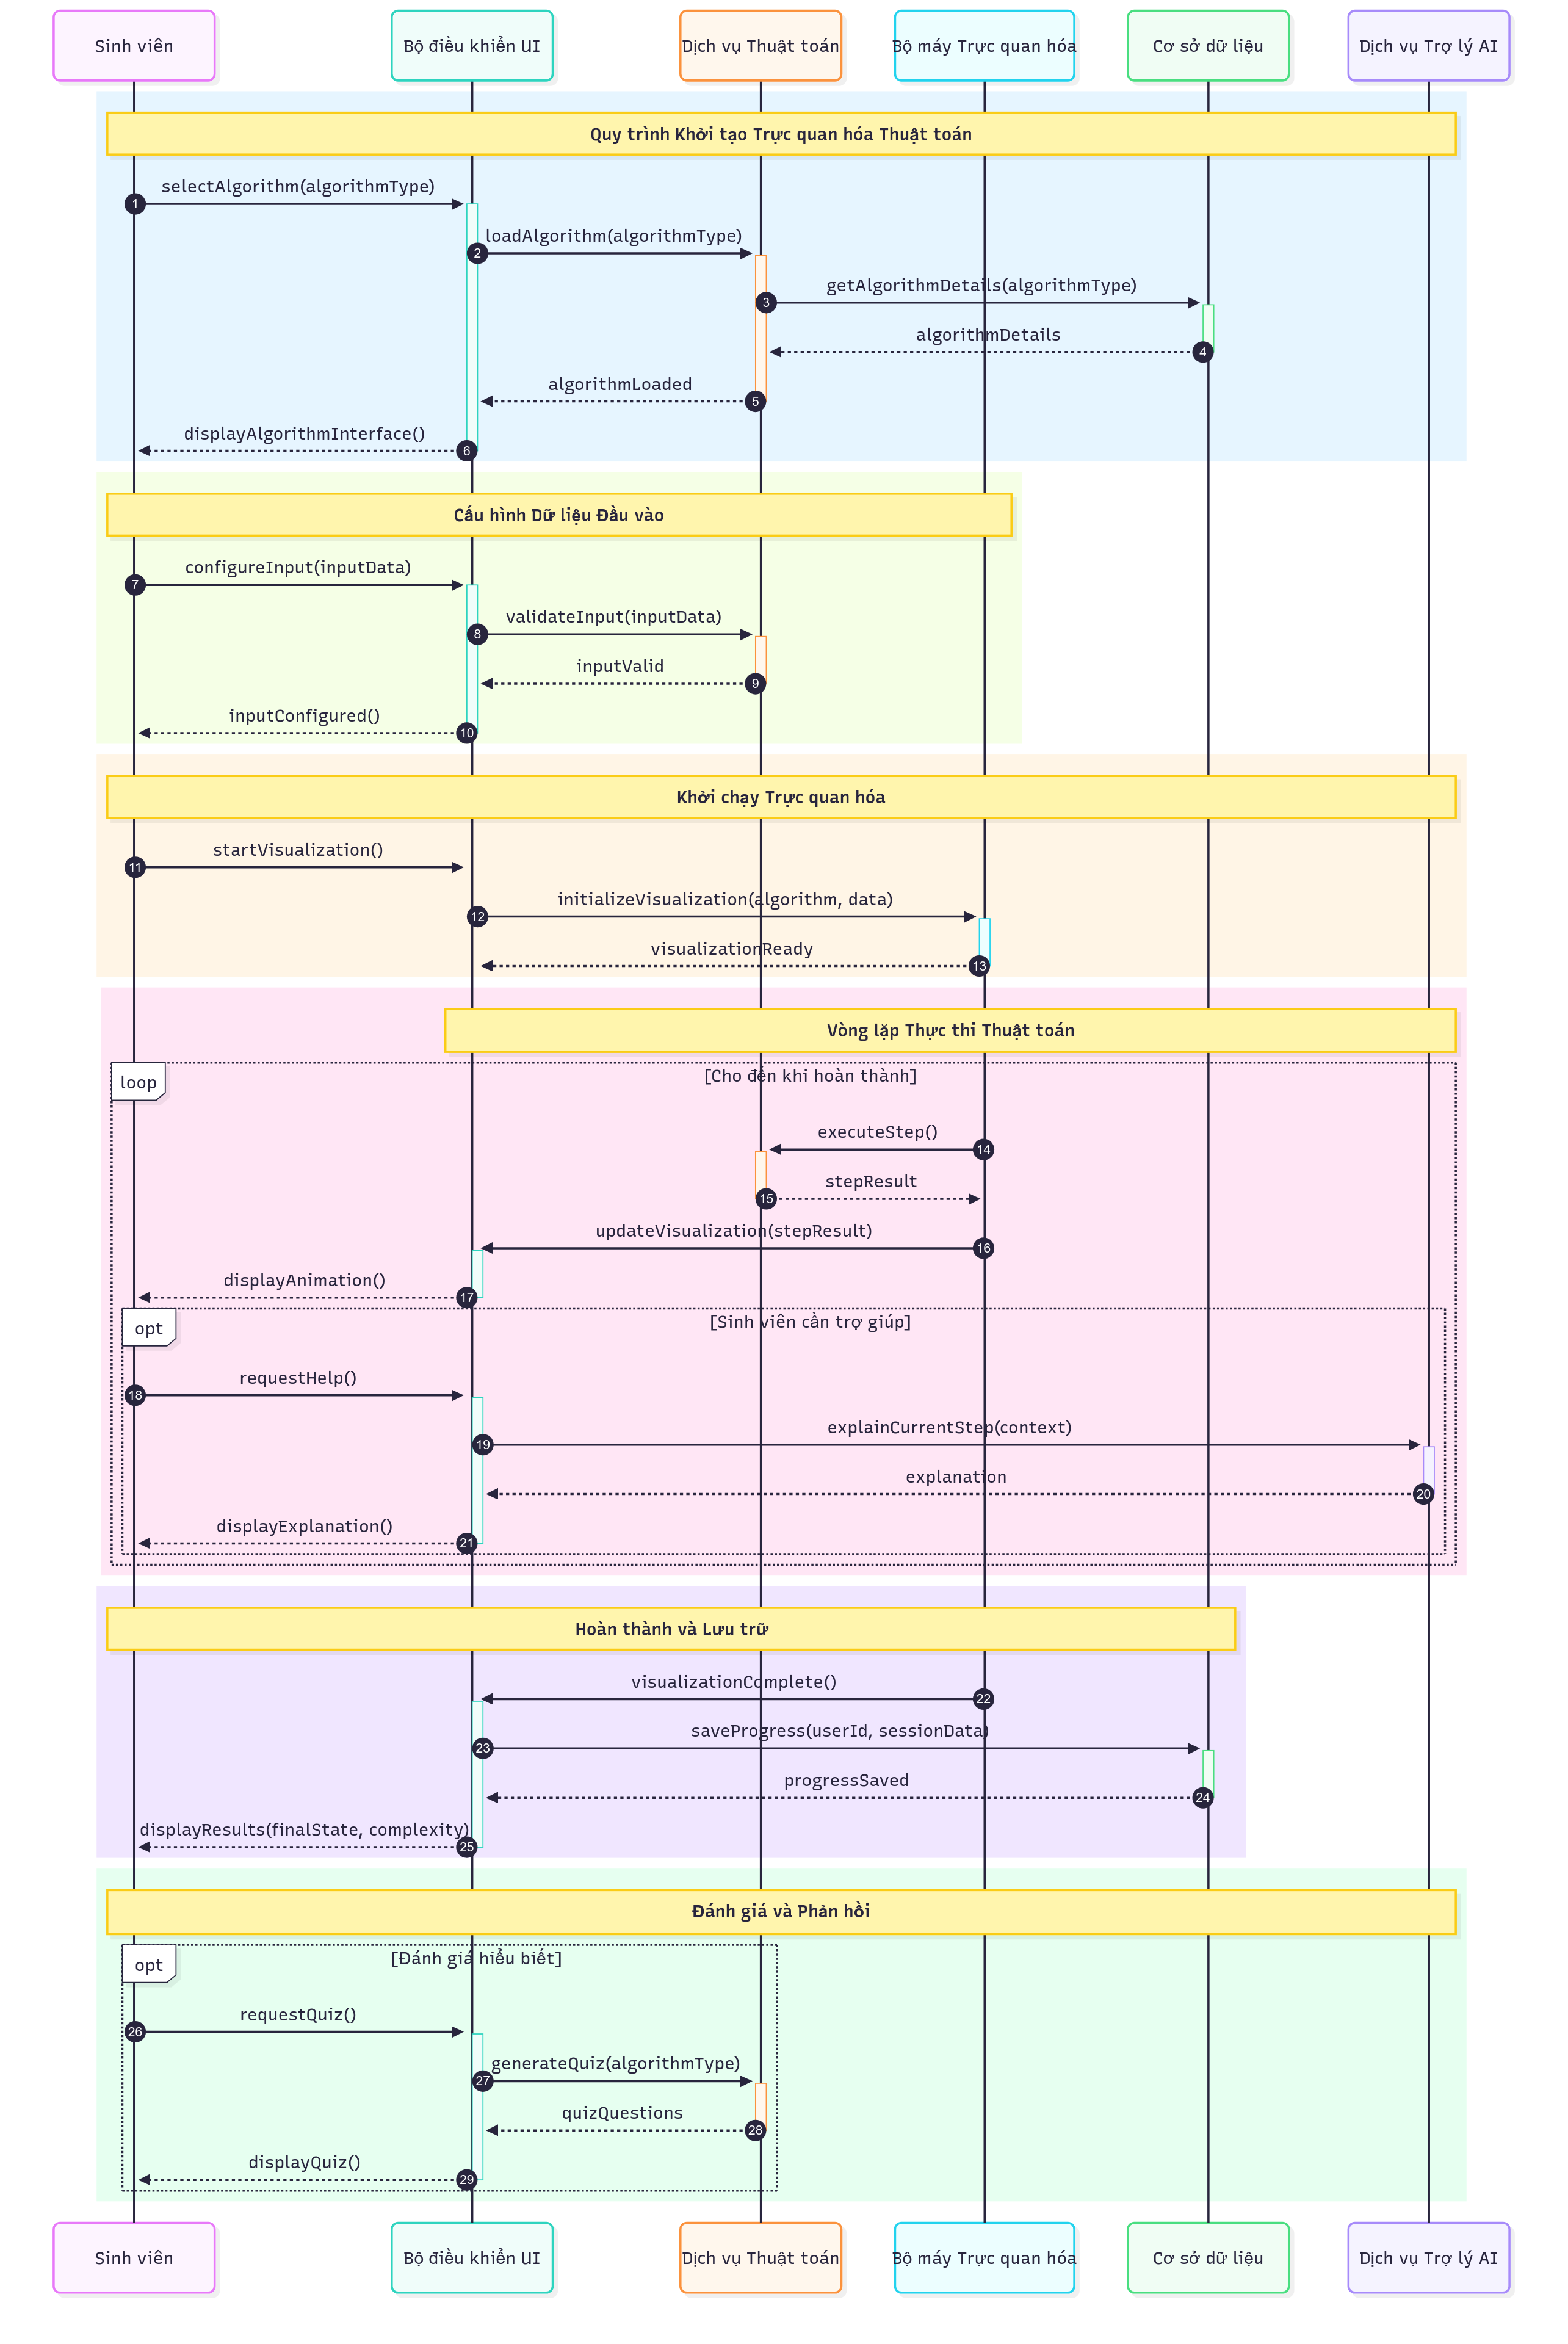
\includegraphics[width=0.95\textwidth]{images/sequence-algorithm-visualization.png}
\caption{Sequence Diagram - Quy trình Trực quan hóa Thuật toán}
\label{fig:sequence-algorithm-visualization}
\end{figure}

\textbf{Các giai đoạn chính:}
\begin{enumerate}
    \item \textbf{Khởi tạo}: Chọn thuật toán và tải cấu hình
    \item \textbf{Cấu hình}: Thiết lập dữ liệu đầu vào và tham số
    \item \textbf{Thực thi}: Chạy thuật toán theo từng bước với trực quan hóa
    \item \textbf{Tương tác}: Hỗ trợ AI khi cần thiết
    \item \textbf{Hoàn thành}: Lưu tiến độ và hiển thị kết quả
\end{enumerate}

\subsection{Sequence Diagram: Tương tác Trợ lý AI}
\label{subsec:ai-assistant-sequence}

Biểu đồ này chi tiết hóa cách thức hoạt động của hệ thống AI Assistant, từ khởi tạo phiên làm việc đến cung cấp khuyến nghị cá nhân hóa.

\begin{figure}[H]
\centering
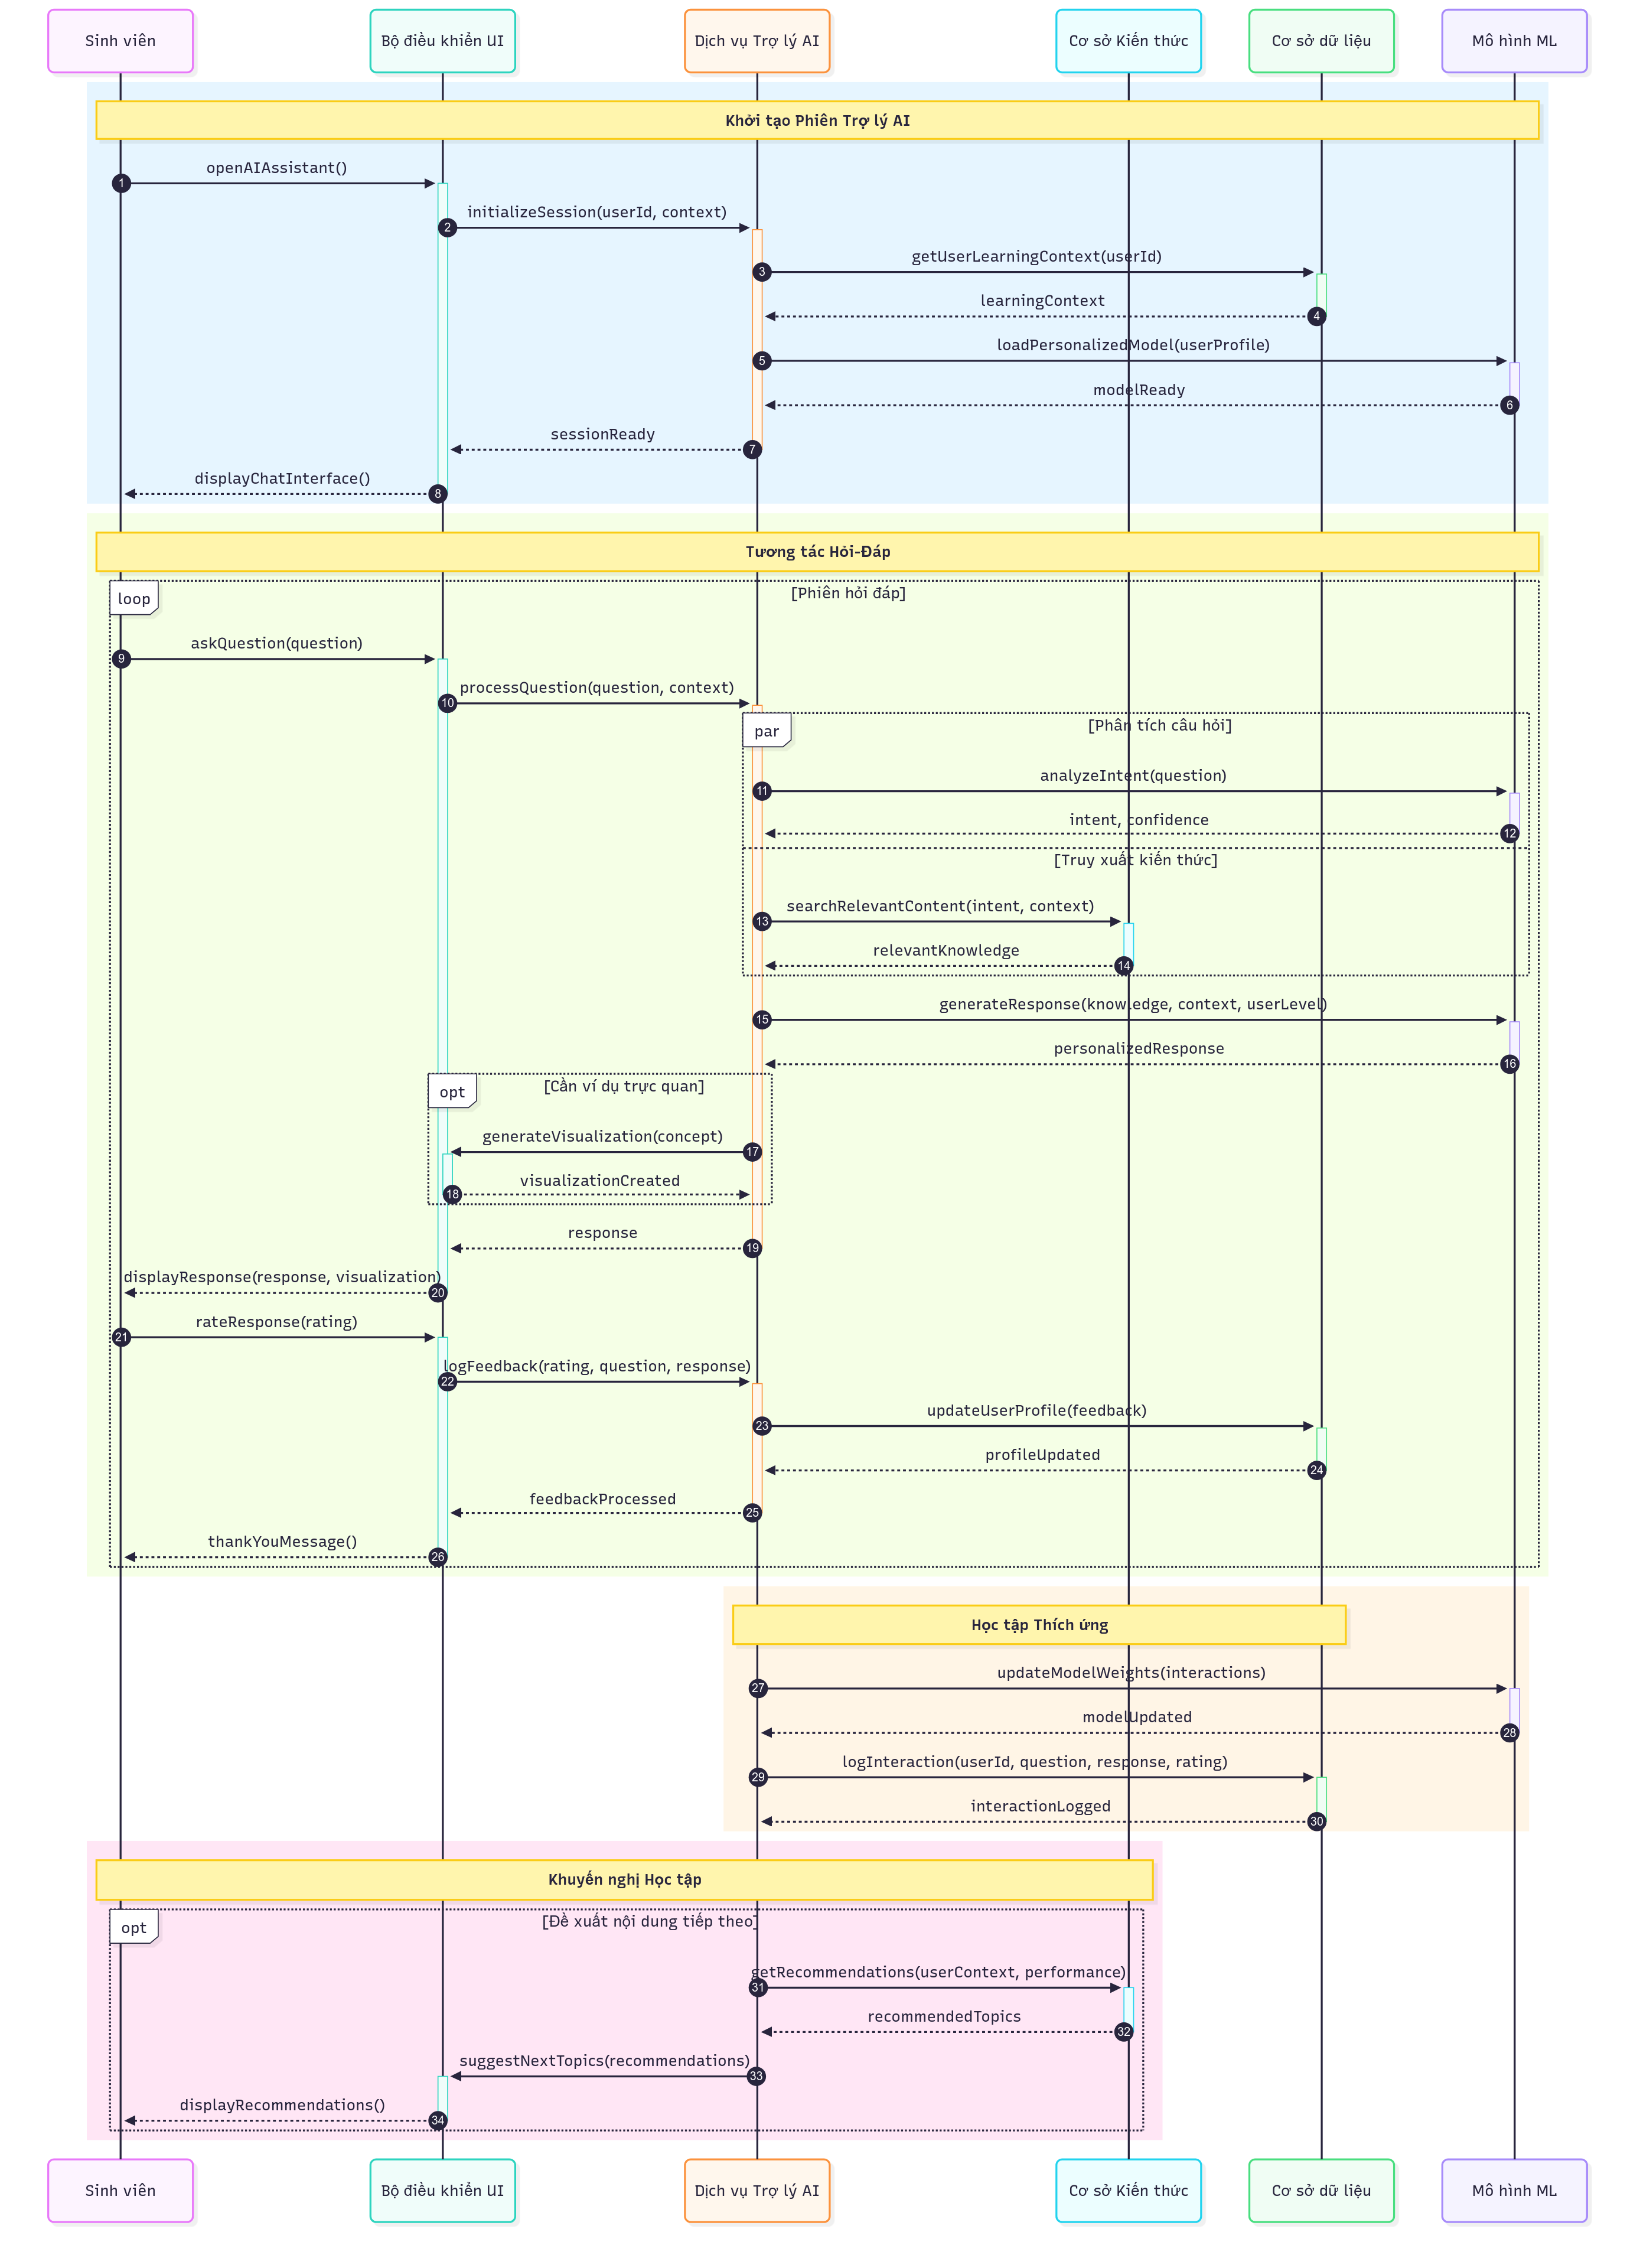
\includegraphics[width=0.95\textwidth]{images/sequence-ai-assistant.png}
\caption{Sequence Diagram - Tương tác Trợ lý AI}
\label{fig:sequence-ai-assistant}
\end{figure}

\textbf{Đặc điểm nổi bật:}
\begin{itemize}
    \item \textbf{Cá nhân hóa}: AI điều chỉnh phản hồi dựa trên profile người học
    \item \textbf{Xử lý song song}: Phân tích intent và truy xuất kiến thức đồng thời
    \item \textbf{Học thích ứng}: Cập nhật model dựa trên feedback của người dùng
    \item \textbf{Trực quan hóa tích hợp}: Tạo visualization để minh họa khái niệm
\end{itemize}

\subsection{Sequence Diagram: Hệ thống Đánh giá}
\label{subsec:assessment-sequence}

Mô tả quy trình đánh giá thích ứng với khả năng điều chỉnh độ khó theo thời gian thực.

\begin{figure}[H]
\centering
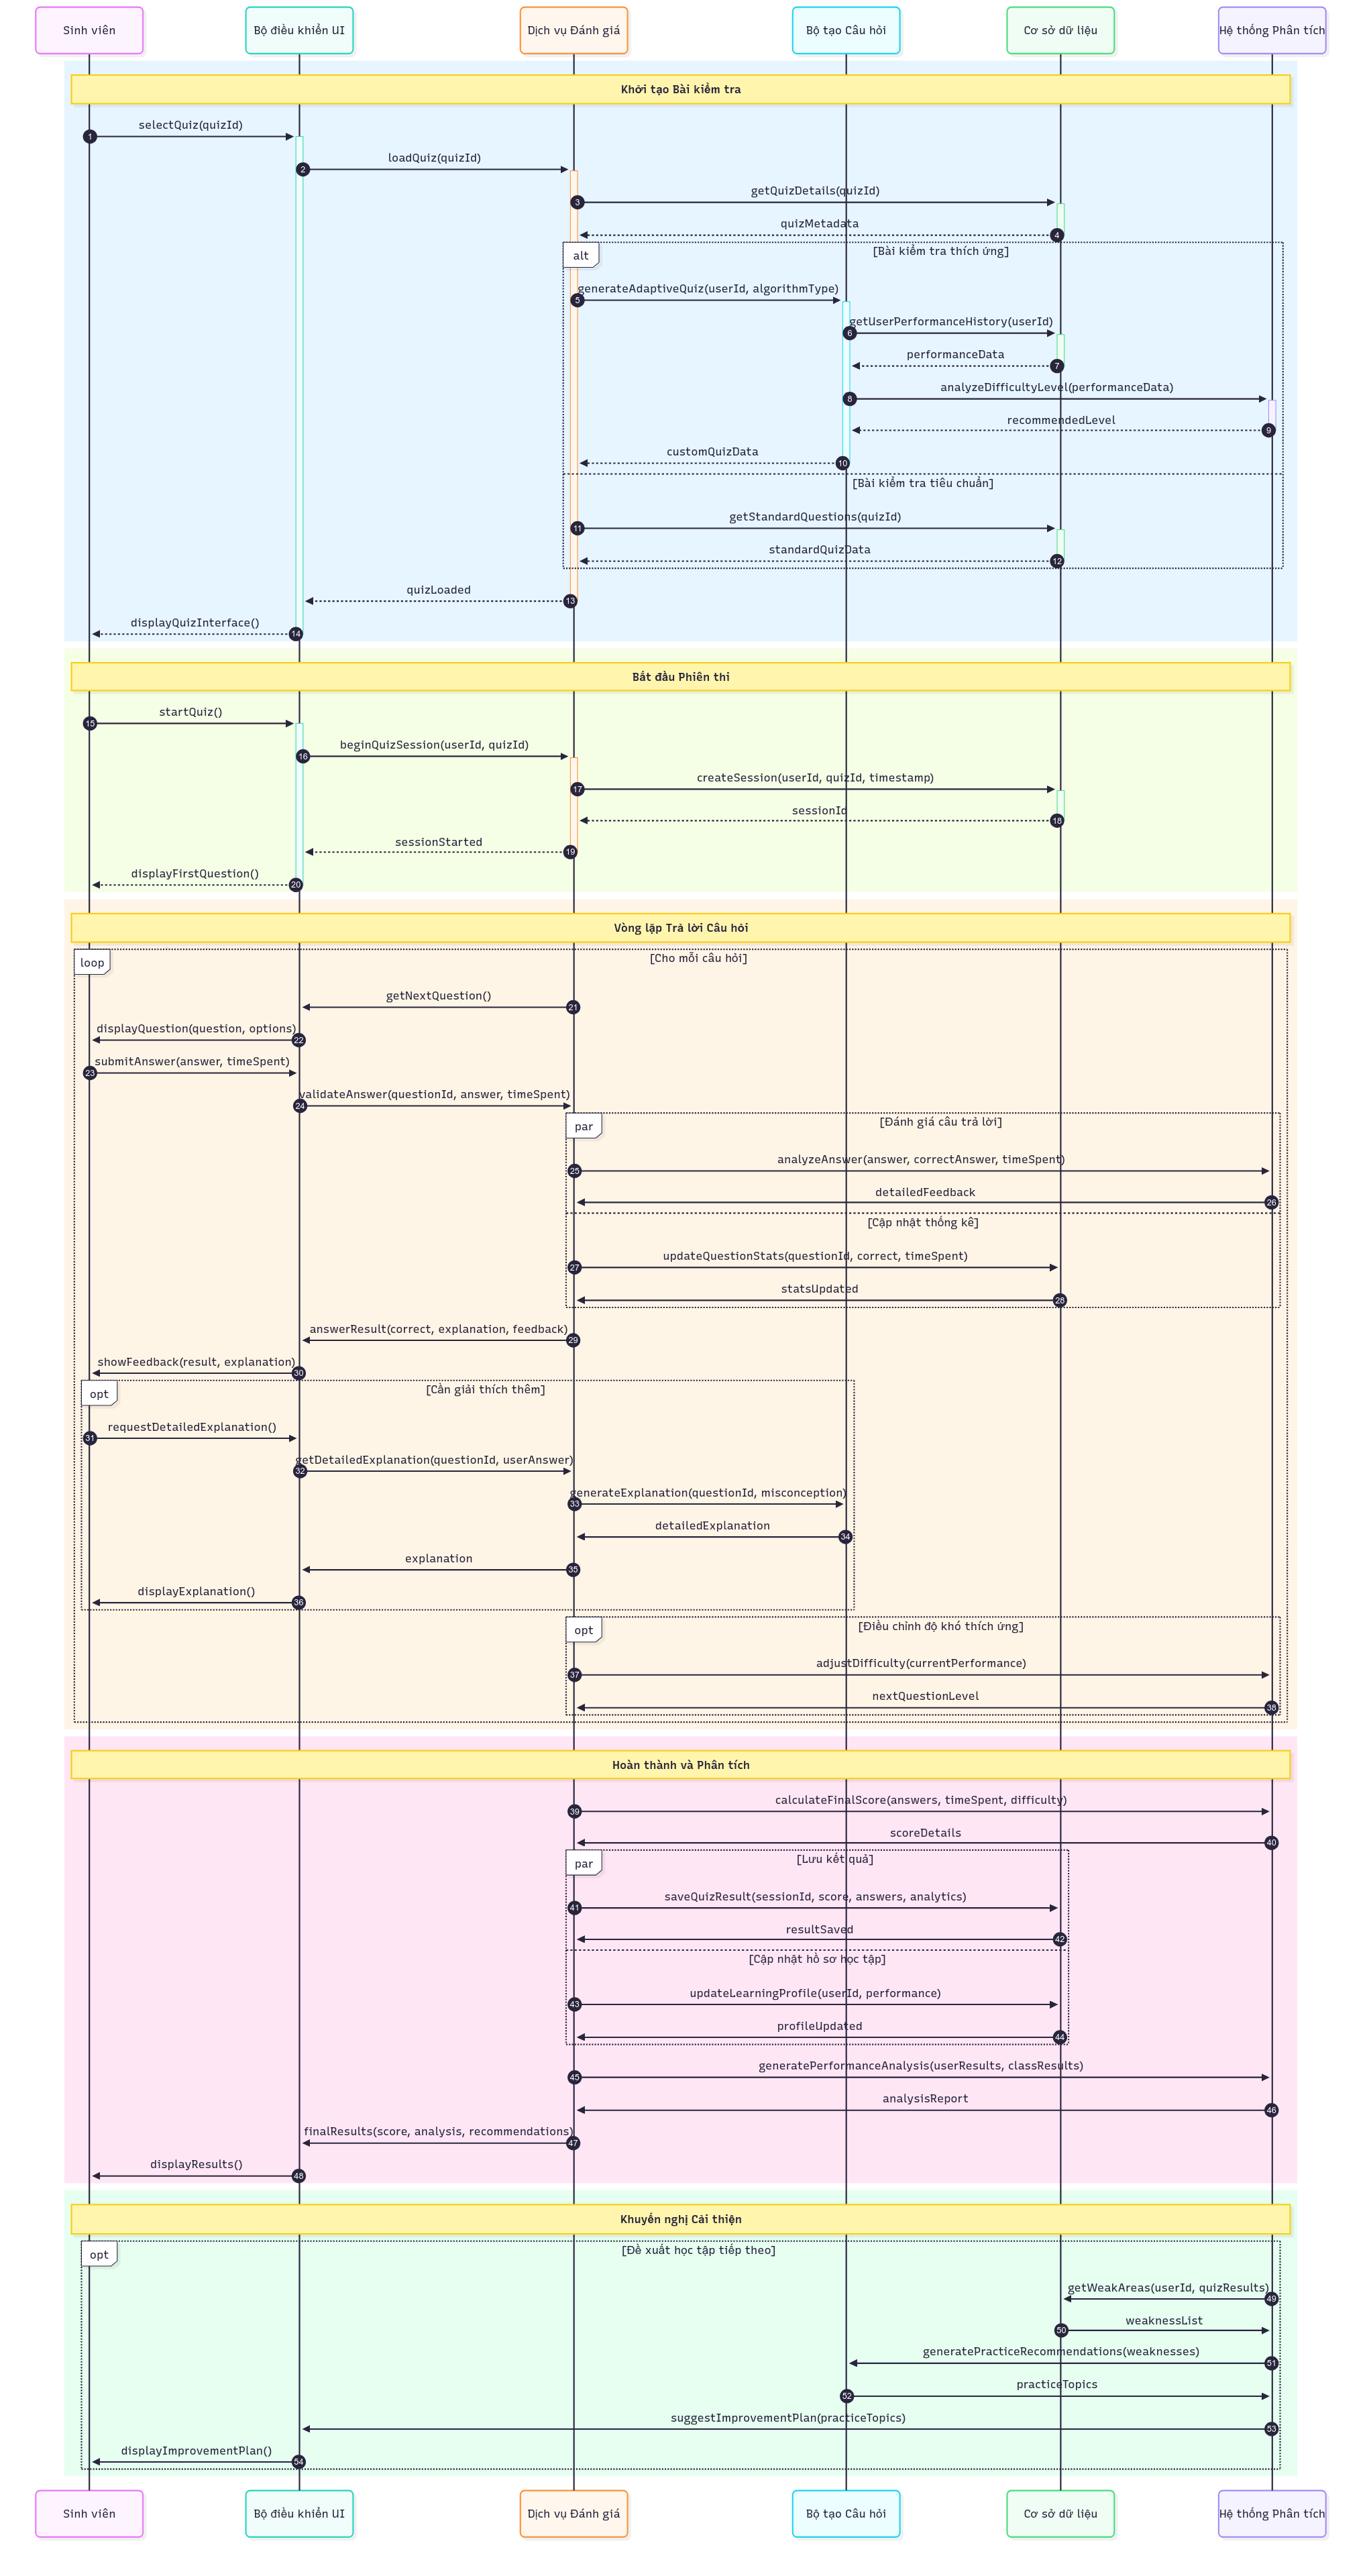
\includegraphics[width=0.95\textwidth]{images/sequence-assessment-system.png}
\caption{Sequence Diagram - Hệ thống Đánh giá}
\label{fig:sequence-assessment-system}
\end{figure}

\textbf{Tính năng tiên tiến:}
\begin{itemize}
    \item \textbf{Đánh giá thích ứng}: Điều chỉnh độ khó dựa trên hiệu suất hiện tại
    \item \textbf{Phân tích chi tiết}: Đánh giá sâu về thời gian và pattern trả lời
    \item \textbf{Feedback tức thì}: Giải thích chi tiết cho từng câu trả lời
    \item \textbf{Khuyến nghị cải thiện}: Đề xuất lộ trình học cụ thể
\end{itemize}

\subsection{Sequence Diagram: Tương tác Hệ thống Tổng thể}
\label{subsec:complete-system-sequence}

Biểu đồ tổng hợp mô tả luồng tương tác hoàn chỉnh từ đăng nhập đến hoàn thành phiên học.

\begin{figure}[H]
\centering
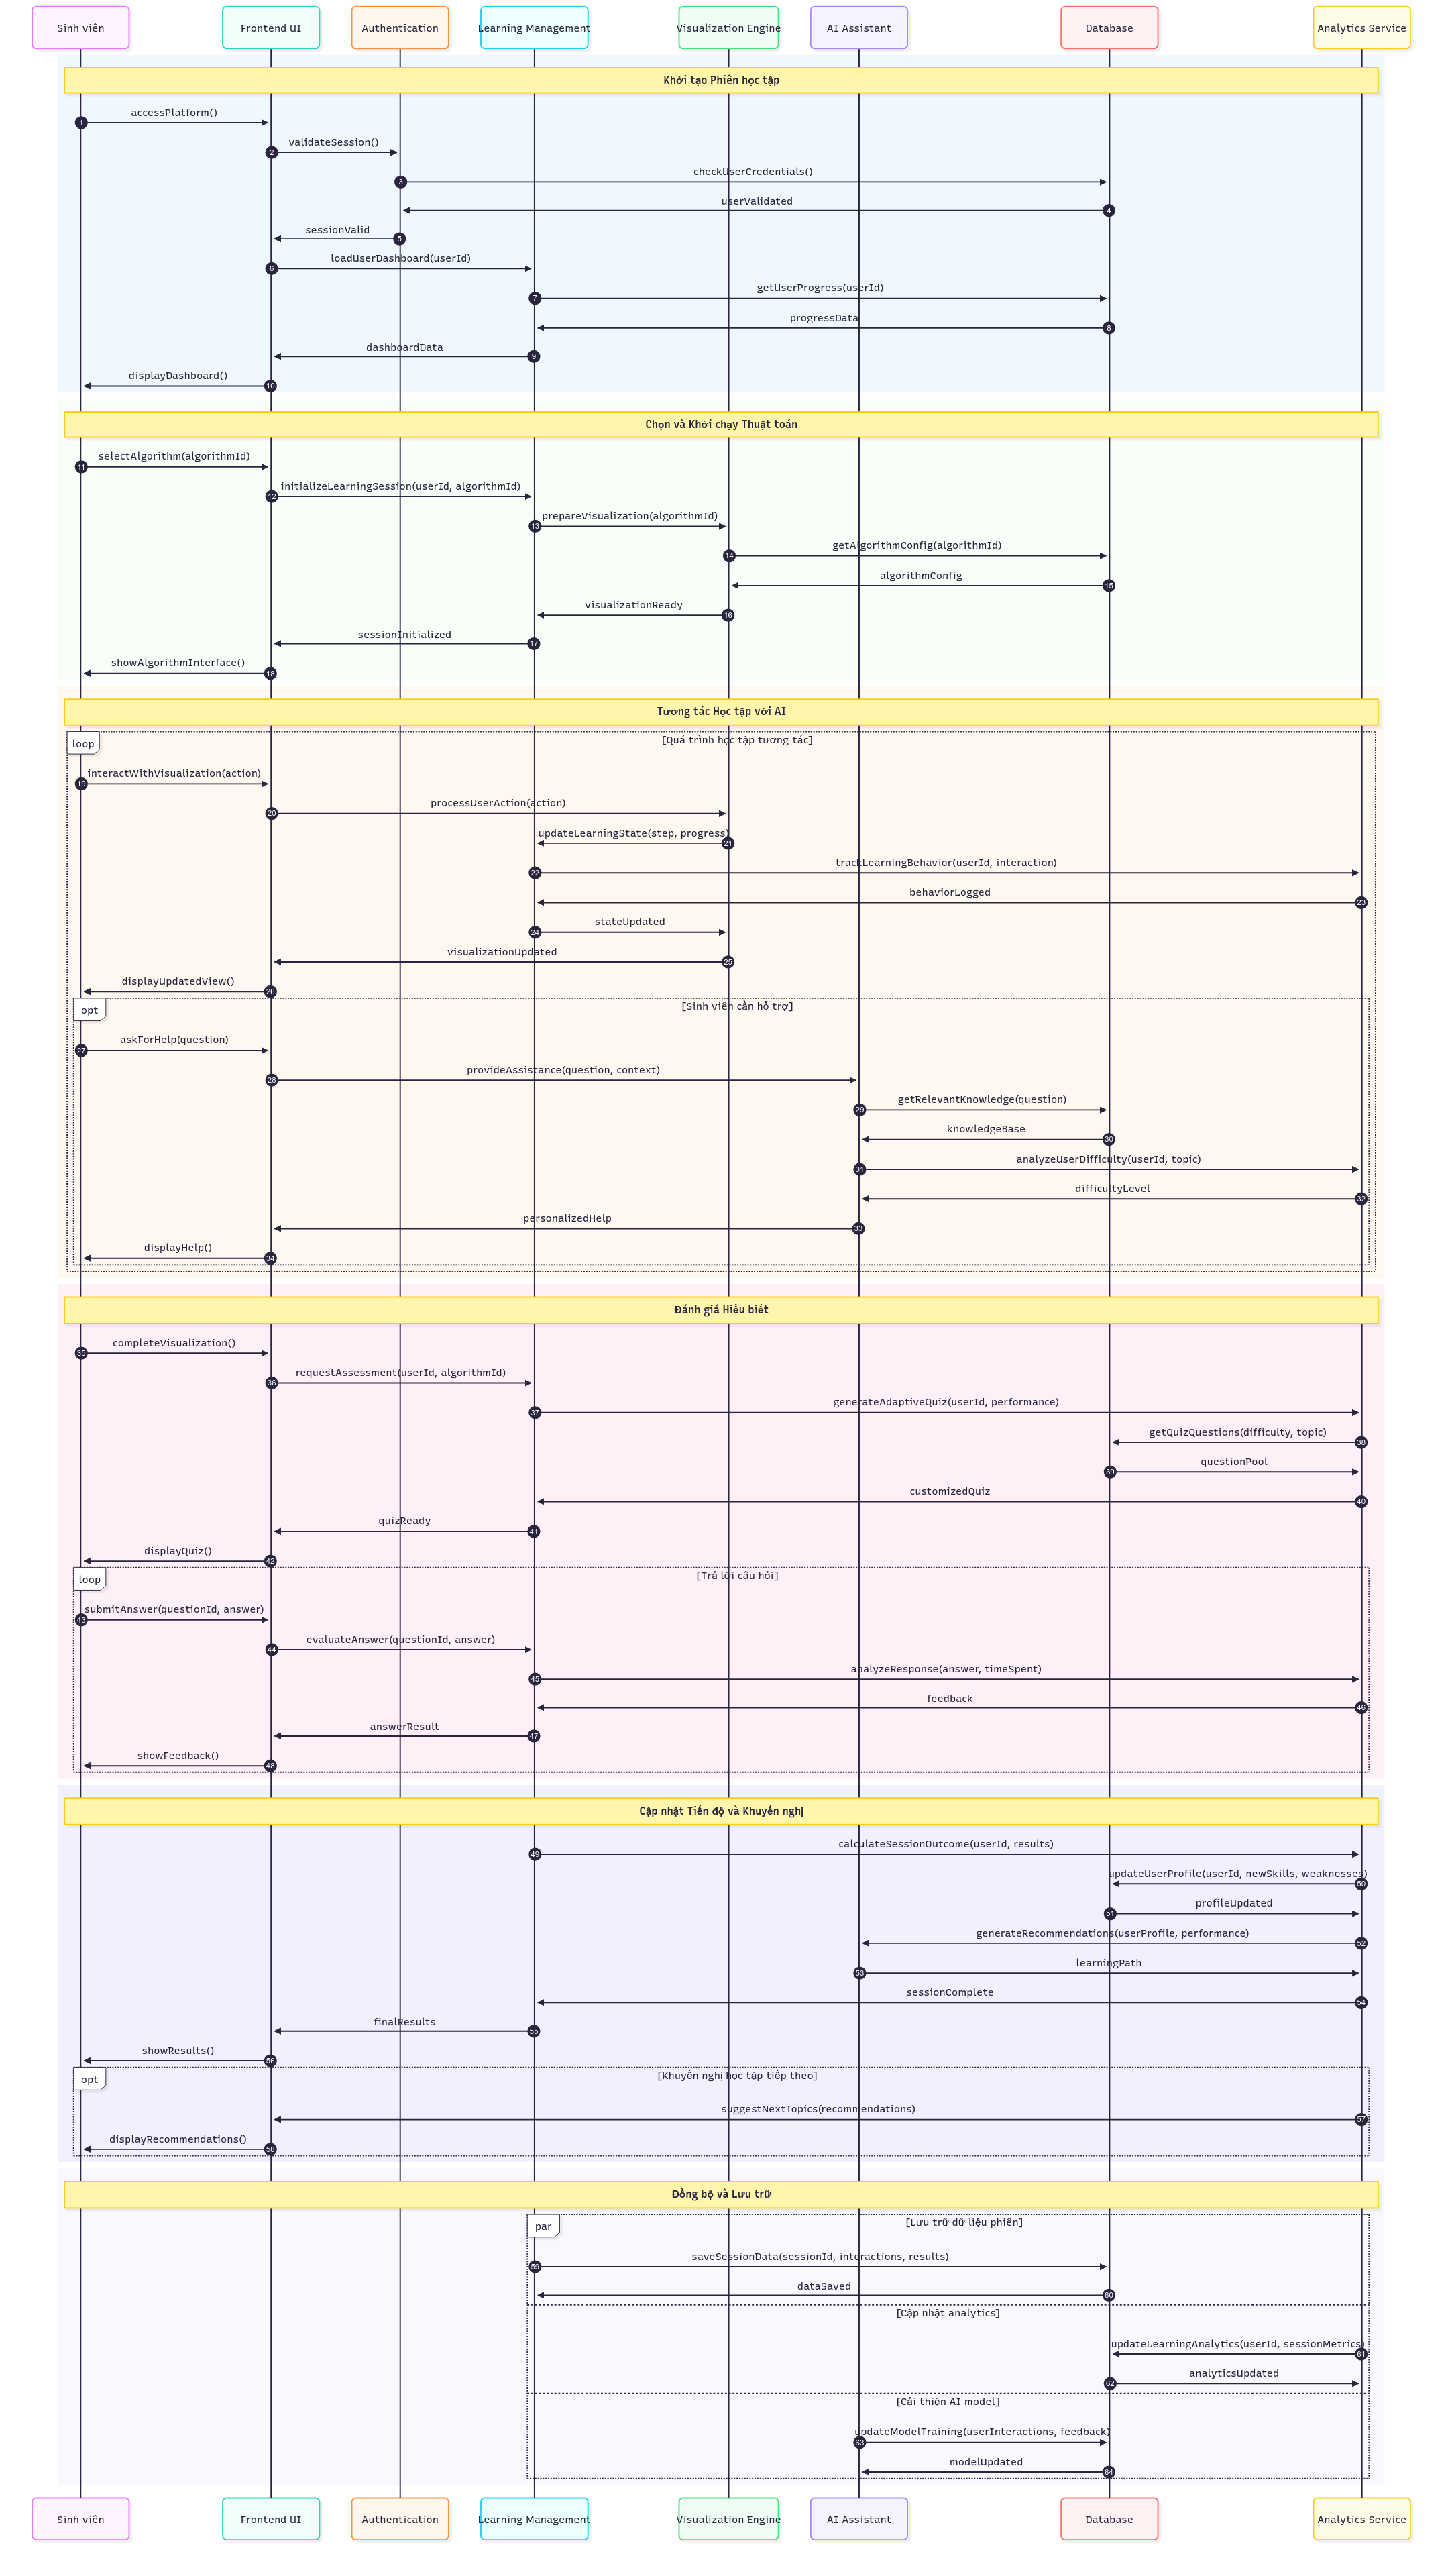
\includegraphics[width=0.95\textwidth]{images/sequence-complete-system.png}
\caption{Sequence Diagram - Hệ thống Hoàn chỉnh}
\label{fig:sequence-complete-system}
\end{figure}

\textbf{Kiến trúc tích hợp:}
\begin{itemize}
    \item \textbf{Authentication}: Quản lý phiên và bảo mật
    \item \textbf{Learning Management}: Điều phối toàn bộ quá trình học
    \item \textbf{Analytics Service}: Thu thập và phân tích dữ liệu học tập
    \item \textbf{Xử lý song song}: Tối ưu hóa hiệu suất hệ thống
\end{itemize}
\end{enumerate}

\subsection{Chuỗi Xử lý Lỗi}

\subsubsection{Chuỗi Lỗi Xác thực}
\begin{enumerate}
    \item \textbf{Sinh viên → Bộ điều khiển UI:} login(credentials)
    \item \textbf{Bộ điều khiển UI → Dịch vụ Xác thực:} validateCredentials(credentials)
    \item \textbf{Dịch vụ Xác thực → Cơ sở dữ liệu:} checkUserCredentials(credentials)
    \item \textbf{Cơ sở dữ liệu → Dịch vụ Xác thực:} userNotFound/invalidPassword
    \item \textbf{Dịch vụ Xác thực → Bộ điều khiển UI:} authenticationFailed(errorType)
    \item \textbf{Bộ điều khiển UI → Sinh viên:} displayErrorMessage(errorType)
    \item \textbf{Bộ điều khiển UI → Sinh viên:} requestCredentialsAgain()
\end{enumerate}

\subsubsection{Chuỗi Khôi phục Lỗi Hệ thống}
\begin{enumerate}
    \item \textbf{Dịch vụ bất kỳ:} systemError(errorDetails)
    \item \textbf{Bộ xử lý Lỗi:} logError(errorDetails)
    \item \textbf{Bộ xử lý Lỗi → Dịch vụ Giám sát:} reportError(errorDetails)
    \item \textbf{Bộ xử lý Lỗi → Bộ điều khiển UI:} notifyUser(genericErrorMessage)
    \item \textbf{Bộ điều khiển UI → Sinh viên:} displayErrorScreen(recoveryOptions)
    \item \textbf{Bộ xử lý Lỗi:} attemptRecovery()
    \item \textbf{Dịch vụ Dự phòng:} provideFallbackFunctionality()
\end{enumerate}

\section{Phân tích Kiến trúc Hệ thống}
\label{sec:system-architecture}

\subsection{Tổng quan Kiến trúc}
\label{subsec:architecture-overview}

Hệ thống DSA Visualizer được thiết kế theo mô hình kiến trúc 5 tầng để đảm bảo khả năng mở rộng, dễ bảo trì và tối ưu hóa hiệu suất.

\begin{center}
\textbf{[Biểu đồ Kiến trúc Hệ thống]}\\
\textit{Diagram: system-architecture.drawio}
\end{center}

\subsection{Chi tiết các Tầng}

\subsubsection{Tầng UI (Tầng Trình bày)}
\textbf{Công nghệ sử dụng:} Next.js 14, React 18, TypeScript, TailwindCSS

\textbf{Thành phần chính:}
\begin{itemize}
    \item \textbf{Trình trực quan hóa Tương tác:} Hoạt hình thuật toán dựa trên Canvas
    \item \textbf{Bảng điều khiển:} Điều khiển tốc độ, điều hướng từng bước
    \item \textbf{Giao diện Bảng điều khiển:} Theo dõi tiến độ và thống kê người dùng
    \item \textbf{Giao diện Trò chuyện AI:} Trò chuyện thời gian thực với Trợ lý AI
    \item \textbf{Giao diện Đánh giá:} Bài kiểm tra và bài tập thực hành
\end{itemize}

\textbf{Mẫu Thiết kế:}
\begin{itemize}
    \item Kiến trúc dựa trên thành phần
    \item Quản lý trạng thái với Context API
    \item Hook tùy chỉnh cho logic có thể tái sử dụng
    \item Mẫu thiết kế đáp ứng
\end{itemize}

\subsubsection{Tầng Bộ máy Trực quan hóa}
\textbf{Công nghệ sử dụng:} D3.js, Canvas API, WebGL

\textbf{Thành phần Cốt lõi:}
\begin{itemize}
    \item \textbf{Bộ điều khiển Hoạt hình:} Quản lý dòng thời gian và trạng thái hoạt hình
    \item \textbf{Bộ máy Hiển thị:} Hiển thị trực quan hóa hiệu suất cao
    \item \textbf{Bộ xử lý Tương tác:} Xử lý đầu vào người dùng cho trực quan hóa
    \item \textbf{Quản lý Trạng thái:} Theo dõi trạng thái thuật toán và lịch sử
\end{itemize}

\textbf{Các loại Trực quan hóa:}
\begin{itemize}
    \item Trực quan hóa Mảng/Danh sách với mã hóa màu
    \item Cấu trúc Cây với các nút tương tác
    \item Trực quan hóa Đồ thị với hoạt hình cạnh
    \item Khung nhìn So sánh cho nhiều thuật toán
\end{itemize}

\subsubsection{Tầng Dịch vụ Backend}
\textbf{Công nghệ sử dụng:} Node.js, Express.js, TypeScript

\textbf{Kiến trúc Microservices:}
\begin{itemize}
    \item \textbf{Dịch vụ Thuật toán:} Thực thi thuật toán và tạo bước
    \item \textbf{Dịch vụ Người dùng:} Xác thực, quản lý hồ sơ
    \item \textbf{Dịch vụ Học tập:} Theo dõi tiến độ, quản lý phiên
    \item \textbf{Dịch vụ Đánh giá:} Tạo bài kiểm tra, hệ thống chấm điểm
    \item \textbf{Dịch vụ AI:} Xử lý ngôn ngữ tự nhiên, truy xuất kiến thức
    \item \textbf{Dịch vụ Phân tích:} Theo dõi hành vi người dùng, chỉ số hiệu suất
\end{itemize}

\textbf{Thiết kế API:}
\begin{itemize}
    \item API RESTful với tài liệu OpenAPI
    \item Điểm cuối GraphQL cho truy vấn dữ liệu phức tạp
    \item Kết nối WebSocket cho tính năng thời gian thực
    \item Giới hạn tốc độ và middleware bảo mật
\end{itemize}

\subsubsection{Tầng Quản lý Dữ liệu}
\textbf{Công nghệ sử dụng:} MongoDB, Redis, PostgreSQL

\textbf{Chiến lược Cơ sở dữ liệu:}
\begin{itemize}
    \item \textbf{MongoDB:} Hồ sơ người dùng, phiên học tập, siêu dữ liệu thuật toán
    \item \textbf{PostgreSQL:} Dữ liệu có cấu trúc, phân tích, báo cáo
    \item \textbf{Redis:} Lưu trữ phiên, dữ liệu thời gian thực, bảng xếp hạng
\end{itemize}

\textbf{Mô hình Dữ liệu:}
\begin{itemize}
    \item Thực thể Người dùng và Hồ sơ với ánh xạ mối quan hệ
    \item Siêu dữ liệu thuật toán với phân tích độ phức tạp
    \item Tiến độ học tập với theo dõi chi tiết
    \item Kết quả đánh giá với phân tích thống kê
\end{itemize}

\subsubsection{Tầng Hạ tầng}
\textbf{Chiến lược Triển khai:} Container Docker, điều phối Kubernetes

\textbf{Dịch vụ Đám mây:}
\begin{itemize}
    \item \textbf{Tính toán:} Máy chủ web tự động mở rộng
    \item \textbf{Lưu trữ:} Lưu trữ tệp phân tán cho tài sản
    \item \textbf{CDN:} Mạng phân phối nội dung toàn cầu
    \item \textbf{Giám sát:} Giám sát hiệu suất ứng dụng
\end{itemize}

\textbf{Biện pháp Bảo mật:}
\begin{itemize}
    \item Xác thực dựa trên JWT với token làm mới
    \item Thực thi HTTPS với chứng chỉ SSL
    \item Xác thực đầu vào và ngăn chặn SQL injection
    \item Cấu hình Chia sẻ Tài nguyên Có nguồn gốc (CORS)
\end{itemize}

\subsection{Mẫu Tích hợp}

\subsubsection{Kiến trúc Hướng sự kiện}
\begin{itemize}
    \item Sự kiện hành động người dùng kích hoạt cập nhật trực quan hóa
    \item Sự kiện tiến độ cập nhật phân tích học tập
    \item Sự kiện thành tích kích hoạt hệ thống thông báo
    \item Sự kiện lỗi kích hoạt giám sát và cảnh báo
\end{itemize}

\subsubsection{Chiến lược Bộ nhớ đệm}
\begin{itemize}
    \item Bộ nhớ đệm trình duyệt cho tài sản tĩnh
    \item Bộ nhớ đệm Redis cho dữ liệu được truy cập thường xuyên
    \item Bộ nhớ đệm CDN cho hiệu suất toàn cầu
    \item Bộ nhớ đệm cấp ứng dụng cho kết quả tính toán
\end{itemize}

\section{Nguyên tắc Thiết kế và Thực hành Tốt nhất}
\label{sec:design-principles}

\subsection{Triển khai Nguyên tắc SOLID}

\subsubsection{Nguyên tắc Trách nhiệm Duy nhất}
Mỗi lớp và thành phần có một trách nhiệm duy nhất:
\begin{itemize}
    \item VisualizationRenderer chỉ xử lý logic hiển thị
    \item AlgorithmExecutor chỉ xử lý thực thi thuật toán
    \item UserManager chỉ xử lý các hoạt động liên quan đến người dùng
\end{itemize}

\subsubsection{Nguyên tắc Mở/Đóng}
Hệ thống được thiết kế để mở rộng chức năng mà không cần sửa đổi:
\begin{itemize}
    \item Kiến trúc plugin cho các loại thuật toán mới
    \item Hệ thống mở rộng cho trực quan hóa tùy chỉnh
    \item Khung đánh giá có thể cấu hình
\end{itemize}

\subsubsection{Nguyên tắc Thay thế Liskov}
Các lớp trừu tượng và giao diện đảm bảo khả năng thay thế:
\begin{itemize}
    \item Giao diện Algorithm có thể được triển khai bởi bất kỳ loại thuật toán nào
    \item Giao diện Visualizer hỗ trợ nhiều chiến lược hiển thị
    \item Giao diện Assessment phù hợp với các loại bài kiểm tra khác nhau
\end{itemize}

\subsection{Tối ưu hóa Hiệu suất}

\subsubsection{Tối ưu hóa Frontend}
\begin{itemize}
    \item Chia tách mã và tải lười cho các thành phần
    \item Ghi nhớ cho các phép tính tốn kém
    \item Cuộn ảo cho tập dữ liệu lớn
    \item Debouncing cho xử lý đầu vào người dùng
\end{itemize}

\subsubsection{Tối ưu hóa Backend}
\begin{itemize}
    \item Tối ưu hóa truy vấn cơ sở dữ liệu với chỉ mục phù hợp
    \item Gộp kết nối cho kết nối cơ sở dữ liệu
    \item Xử lý bất đồng bộ cho các tác vụ tốn thời gian
    \item Cân bằng tải cho tính khả dụng cao
\end{itemize}

\subsection{Khả năng Tiếp cận và Khả năng Sử dụng}

\subsubsection{Tính năng Khả năng Tiếp cận}
\begin{itemize}
    \item Tuân thủ WCAG 2.1 cho tiêu chuẩn khả năng tiếp cận
    \item Hỗ trợ điều hướng bằng bàn phím
    \item Tương thích với trình đọc màn hình
    \item Chế độ tương phản cao cho khiếm thị
\end{itemize}

\subsubsection{Tính năng Khả năng Sử dụng}
\begin{itemize}
    \item Thiết kế giao diện người dùng trực quan
    \item Tiết lộ dần dần các tính năng phức tạp
    \item Trợ giúp ngữ cảnh và chú giải công cụ
    \item Thiết kế đáp ứng cho nhiều thiết bị
\end{itemize}

\section{Kết luận Chương 3}
\label{sec:chapter3-conclusion}

Chương 3 đã phân tích chi tiết hệ thống DSA Visualizer từ góc độ kiến trúc kỹ thuật và thiết kế. Các điểm chính bao gồm:

\subsection{Phân tích Use Case}
Đã định nghĩa và mô tả chi tiết các use case chính của hệ thống, bao gồm học tập thuật toán, thực hành tương tác, và tư vấn trợ lý AI. Mỗi use case được tài liệu hóa với định dạng bảng chi tiết theo chuẩn học thuật.

\subsection{Phân tích Biểu đồ UML}
\begin{itemize}
    \item \textbf{Biểu đồ Lớp:} Thiết kế OOP với các mẫu thiết kế phù hợp
    \item \textbf{Biểu đồ Hoạt động:} Mô tả chi tiết quy trình hoạt động và luồng quyết định
    \item \textbf{Biểu đồ Tuần tự:} Phân tích tương tác giữa đối tượng theo dòng thời gian
\end{itemize}

\subsection{Kiến trúc Hệ thống}
Thiết kế kiến trúc 5 tầng đảm bảo:
\begin{itemize}
    \item Khả năng mở rộng cho việc mở rộng trong tương lai
    \item Khả năng bảo trì với thiết kế mô-đun
    \item Tối ưu hóa hiệu suất với chiến lược bộ nhớ đệm
    \item Bảo mật với các biện pháp bảo vệ toàn diện
\end{itemize}

\subsection{Xuất sắc Kỹ thuật}
Áp dụng nguyên tắc SOLID, mẫu thiết kế, và thực hành tốt nhất để tạo ra một hệ thống mạnh mẽ và chuyên nghiệp.

Tiếp theo, Chương 4 sẽ tập trung vào chi tiết triển khai và đặc tả kỹ thuật của từng thành phần.
